\documentclass[%
a4paper,
DIV12,
2.5headlines,
bigheadings,
titlepage,
openbib,
twoside,
%draft
]{scrartcl}

%%% PACKAGES
\usepackage{rotating}
\usepackage[ngerman, english]{babel} % zuerst deutsche Silbentrennung
%% FONTS
\usepackage{geometry}
\usepackage[ansinew]{inputenc} % deutschen Umlaute
\usepackage[T1]{fontenc}
\usepackage{mathpazo}
\usepackage{amsmath}
\usepackage[scaled=.95]{helvet}
\usepackage{courier}
\usepackage[gen]{eurosym}
\usepackage{courier}
\usepackage{scrpage2}
\usepackage{graphicx}
\usepackage{xcolor}
\usepackage{multirow}
\usepackage{varioref}
\usepackage{babelbib}
\usepackage{makeidx}
\usepackage{tabularx}
\usepackage{hyperref}
\usepackage{wrapfig}
\usepackage{listings}
\usepackage{booktabs}
\usepackage{ctable}
\usepackage{multirow}
\usepackage{nomencl}
\usepackage{subfig}
\usepackage{lscape}
\usepackage{tikz}
\usepackage{pgfplots}
\usepackage{siunitx}
\usepackage{hvfloat}
\usepackage{afterpage}
%\usepackage{showframe}
\usepackage[titletoc]{appendix}
\usetikzlibrary{er}
\usetikzlibrary{positioning}

%\usepackage{nomencl}
\makenomenclature
\renewcommand{\nomname}{Abkürzungverzeichnis}
\setlength{\nomlabelwidth}{.25\hsize}
\setlength{\nomitemsep}{-\parsep}
%\usepackage{tex4ht}
\pagestyle{scrheadings} % Seitenkopf
%\usepackage[explicit]{titlesec}
\geometry{a4paper, top=55mm, left=40mm, right=35mm, bottom=40mm,
headsep=10mm, footskip=22mm}
\linespread {1.25}

\setcounter{secnumdepth}{2} % only chapter and sections will be numbered
\setcounter{tocdepth}{2}    % entries down to \subsubsections in the TOC
\renewcommand*\lstlistingname{Code-Beispiel}

% code block settings
\definecolor{light-gray}{gray}{0.95}
\definecolor{atcolor}{HTML}{4271AE}
\lstdefinelanguage{JavaScript}{
  %keywords=[1]{for, typeof, new, true, false, catch, function, return, null, catch, switch, var, if, in, while, do, else, case, break, SQL, push, data, length, execute},
	keywords=[1]{break, case, class, catch, const, continue, debugger, default, delete, do, else, export, extends, finally, for, function, if, import, in, instanceof, let, new, return, super, switch, this, throw, try, typeof, var, void, while, with, yield},
  %keywordstyle=[1]\color{blue}\bfseries,
	keywordstyle=[1]\color[HTML]{8959A8}\bfseries,
  sensitive=false,
  comment=[s]{//},
  morecomment=[s]{/*}{*/},
  morecomment=[s]{(/}{/g},
  morecomment=[s]{(/}{/g},
  morestring=[b]',
  morestring=[b]",
	stringstyle=\color[HTML]{718C00}\ttfamily
}

\lstdefinelanguage{JavaScriptSQL}{
  %keywords=[1]{for, typeof, new, true, false, catch, function, return, null, catch, switch, var, if, in, while, do, else, case, break, SQL, push, data, length, execute},
	keywords=[3]{break, class, catch, const, continue, debugger, default, delete, do, else, export, extends, finally, for, function, if, import,  instanceof, let, new, return, super, switch, this, throw, try, typeof, var, void, while, with, yield},
  keywords=[2]{ALL, ALTER, AS, BEFORE, BEGIN, BOTH, CASE, CHAR, CONDITION, CONNECT, CROSS, CUBE, CURRENT_CONNECTION, CURRENT_DATE, CURRENT_SCHEMA, CURRENT_TIME, CURRENT_TIMESTAMP, CURRENT_USER, CURRENT_UTCDATE, CURRENT_UTCTIME, CURRENT_UTCTIMESTAMP, CURRVAL, CURSOR, DECLARE, DISTINCT, ELSE, ELSEIF, ELSIF, END, EXCEPT, EXCEPTION, EXEC, FOR, FROM, FULL, GROUP, HAVING, IF, IN, INNER, INOUT, INTERSECT, INTO, IS, JOIN, LEADING, LEFT, LIMIT, LOOP, MINUS, NATURAL, NEXTVAL, NULL, ON, ORDER, OUT, PRIOR, RETURN, RETURNS, REVERSE, RIGHT, ROLLUP, ROWID, SELECT, SET, SQL, START, SYSDATE, SYSTIME, SYSTIMESTAMP, SYSUUID, TOP, TRAILING, UNION, USING, UTCDATE, UTCTIME, UTCTIMESTAMP, VALUES, WHEN, WHERE, WHILE, WITH, OUTER, BETWEEN, AND, OR},
	keywords=[1]{@},
  %keywordstyle=[1]\color{blue}\bfseries,
	keywordstyle=[1]\color[HTML]{4271AE}\bfseries,
  keywordstyle=[2]\color[HTML]{F5871F}\bfseries,
	keywordstyle=[3]\color[HTML]{8959A8}\bfseries,
  sensitive=false,
  comment=[s]{//},
  morecomment=[s]{/*}{*/},
  morecomment=[s]{(/}{/g},
  morecomment=[s]{(/}{/g},
  %morecomment=[s][\color{atcolor}\bfseries]{@}{\ },
  morestring=[b]',
  morestring=[b]",
	stringstyle=\color[HTML]{718C00}\ttfamily,
	%keywordsprefix=\@,
	keywordsprefix=\@,
	alsoletter=\@,
	%alsoletter=\:,\@,
}
\lstdefinelanguage{JavaScriptSQL2}{
  %keywords=[1]{for, typeof, new, true, false, catch, function, return, null, catch, switch, var, if, in, while, do, else, case, break, SQL, push, data, length, execute},
	keywords=[3]{break, class, catch, const, continue, debugger, default, delete, do, export, extends, finally, for, function, if, import,  instanceof, let, new, return, super, switch, this, throw, try, typeof, var, void, while, with, yield},
  keywords=[2]{ALL, ALTER, AS, BEFORE, BEGIN, BOTH, CASE, CHAR, CONDITION, CONNECT, CROSS, CUBE, CURRENT_CONNECTION, CURRENT_DATE, CURRENT_SCHEMA, CURRENT_TIME, CURRENT_TIMESTAMP, CURRENT_USER, CURRENT_UTCDATE, CURRENT_UTCTIME, CURRENT_UTCTIMESTAMP, CURRVAL, CURSOR, DECLARE, DISTINCT, ELSE, ELSEIF, ELSIF, END, EXCEPT, EXCEPTION, EXEC, FOR, FROM, FULL, GROUP, HAVING, IF, IN, INNER, INOUT, INTERSECT, INTO, IS, JOIN, LEADING, LEFT, LIMIT, LOOP, MINUS, NATURAL, NEXTVAL, NULL, ON, ORDER, OUT, PRIOR, RETURN, RETURNS, REVERSE, RIGHT, ROLLUP, ROWID, SELECT, SET, SQL, START, SYSDATE, SYSTIME, SYSTIMESTAMP, SYSUUID, TOP, TRAILING, UNION, USING, UTCDATE, UTCTIME, UTCTIMESTAMP, VALUES, WHEN, WHERE, WHILE, WITH, OUTER, BETWEEN, AND, INSERT, THEN},
	keywords=[1]{@},
  %keywordstyle=[1]\color{blue}\bfseries,
	keywordstyle=[1]\color[HTML]{4271AE}\bfseries,
  keywordstyle=[2]\color[HTML]{F5871F}\bfseries,
	keywordstyle=[3]\color[HTML]{8959A8}\bfseries,
  sensitive=false,
  comment=[s]{//},
  morecomment=[s]{/*}{*/},
  morecomment=[s]{(/}{/g},
  morecomment=[s]{(/}{/g},
  %morecomment=[s][\color{atcolor}\bfseries]{@}{\ },
  morestring=[b]',
  morestring=[b]",
	stringstyle=\color[HTML]{718C00}\ttfamily,
	keywordsprefix=\@,
	alsoletter=\@,
}

\lstdefinelanguage{mySQL}{
  language=SQL,
  keywordstyle=\color[HTML]{F5871F},
  %deletekeywords={table},
  morekeywords={[1]{schema}},
  %keywordstyle={[2]{\color{red}}},
}


\lstset{
  backgroundcolor=\color{light-gray},   % choose the background color; you must add \usepackage{color} or \usepackage{xcolor}
  basicstyle=\footnotesize,        			% the size of the fonts that are used for the code
  breakatwhitespace=false,         			% sets if automatic breaks should only happen at whitespace
  %breaklines=true,                 			% sets automatic line breaking
  captionpos=b,                    			% sets the caption-position to bottom
  commentstyle=\color{gray},    			  % comment style
  %deletekeywords={...},            	  % if you want to delete keywords from the given language
  %escapeinside={\%*}{*)},          	  % if you want to add LaTeX within your code
  extendedchars=true,              			% lets you use non-ASCII characters; for 8-bits encodings only, does not work with UTF-8
  %frame=single,                    			% adds a frame around the code
  %keepspaces=true,                 			% keeps spaces in text, useful for keeping indentation of code (possibly needs columns=flexible)
  keywordstyle=\color{blue},       			% keyword style
  %language=Octave,                 			% the language of the code
  %morekeywords={*,...},            			% if you want to add more keywords to the set
  numbers=left,                    			% where to put the line-numbers; possible values are (none, left, right)
  numbersep=5pt,                   			% how far the line-numbers are from the code
  %numberstyle=\tiny\color{mygray}, 			% the style that is used for the line-numbers
  %rulecolor=\color{black},         			% if not set, the frame-color may be changed on line-breaks within not-black text (e.g. comments (green here))
  showspaces=false,                			% show spaces everywhere adding particular underscores; it overrides 'showstringspaces'
  showstringspaces=false,          			% underline spaces within strings only
  showtabs=false,                  			% show tabs within strings adding particular underscores
  stepnumber=1,                    			% the step between two line-numbers. If it's 1, each line will be numbered
  %stringstyle=\color{mymauve},     			% string literal style
  tabsize=2,                       			% sets default tabsize to 2 spaces
  %title=\lstname                   			% show the filename of files included with \lstinputlisting; also try caption instead of title
}

%%% COMMANDS

	%%%%%%%%%%%%%%%%%%
	% Autor eintragen
	\newcommand{\theauthor}{Frank Blechschmidt}
	%%%%%%%%%%%%%%%%%%
	% Matrikelnummer eintragen
	\newcommand{\matrnr}{759762}
	%%%%%%%%%%%%%%%%%%
	% Titel eintragen
	\newcommand{\thetitle}{Konzepte zur Erstellung datenbewusster Tests anhand eines Fallbeispiels aus dem Unternehmenssektor}
	\newcommand{\thesubtitle}{Guided Creation of Data-Aware Test Cases Based on a Real World Business Use Case}
	% \newcommand{\thesubtitle}{conception}

%%% COLORS
% Rot
\definecolor{hpired}{rgb}{0.686,0,0.204}
% Orange
\definecolor{hpiorange}{rgb}{0.867,0.380,0.031}	
% Gelb
\definecolor{hpiyellow}{rgb}{0.965,0.659,0}			%100 
\colorlet{hpiyellow2}{hpiyellow!60!white}				% 60
\colorlet{hpiyellow3}{hpiyellow!40!white}				% 40
\colorlet{hpiyellow4}{hpiyellow!20!white}				% 20
% Grau
\definecolor{hpigrey}{rgb}{0.376,0.408,0.420}		%100
\colorlet{hpigrey2}{hpigrey!70!white}						% 70
\colorlet{hpigrey3}{hpigrey!50!white}						% 50
\colorlet{hpigrey4}{hpigrey!20!white}						% 20
% Blau
\definecolor{hpiblue}{rgb}{0,0.478,0.620}				%100
\colorlet{hpiblue2}{hpiblue!60!white}						% 60
\colorlet{hpiblue3}{hpiblue!40!white}						% 40
\colorlet{hpiblue4}{hpiblue!15!white}						% 15

%%% OTHER INPUTS
\usepackage{array}
\usepackage{supertabular}
\usepackage{colortbl}

\newcounter{todocounter}
\setcounter{todocounter}{0}
\newcounter{authcounter}
\setcounter{authcounter}{0}
%%% BEGIN Write TODO in File
\def\getdefhelp#1->#2\endhelp{#2}
\def\getdef#1#2{\edef#2{\expandafter\getdefhelp\meaning#1\endhelp}}
\newwrite\TodoDatei
\newwrite\AuthorDatei
\openout\AuthorDatei=author.out
\newcommand{\WriteTodo}[2]{%
	\def\Cont{#2}
	\getdef\Cont\Content
	\edef\WriteIndex{%
		\write\TodoDatei{\string\textcolor{#1}{\string\textbf{\Content}}\string\dotfill\string\pageref{todo:\thetodocounter}}}%
	\WriteIndex}

\newcommand{\WriteAuthor}[1]{%
	\def\Cont{#1}
	\getdef\Cont\Content
	\edef\WriteAuth{\write\AuthorDatei{\Content\string\dotfill\string\ref{auth:\theauthcounter}}}
	\WriteAuth}


%%% END Write TODO in File

% command \BibTeX
\def\BibTeX{{\rm B\kern-.05em{\sc i\kern-.025em b}\kern-.08em
     T\kern-.1667em\lower.7ex\hbox{E}\kern-.125emX}} 

% day in journal: \journalday{date}{titel}{persons}{aktivity}
\newcommand{\journalday}[4]{%
\def\titleTmp{#2}
\subsection*{#1\ifx\titleTmp\empty{}\else{: #2}\fi}
\begin{center}
\begin{tabularx}{\textwidth}{@{}lX@{}}
	Anwesende: & #3\\
	Vorgang: & #4
\end{tabularx}
\end{center}
}

% errorreport: \errorreport{date}{error}{reason}{solution}
\newcommand{\errorreport}[4]{%
\def\dateTmp{#1}
\def\errorTmp{#2}
\def\reasonTmp{#3}
\def\solutionTmp{#4}
\ifx\errorTmp\empty{}\else{%
\subsection*{\ifx\dateTmp\empty{}\else{\hfill(#1)\\}\fi Problem: #2}%
{\begin{center}%
\vskip-1ex%
\begin{tabularx}{\linewidth}{@{}lX@{}}
	Ursache: & \ifx\reasonTmp\empty{unbekannt}\else{#3}\fi\\
	Lösung: & \ifx\solutionTmp\empty{unbekannt}\else{#4}\fi\\
\end{tabularx}%
\end{center}%
}}\fi}

% code: \code[textcolor]{backgroundcolor}{content}
\newcommand{\code}[3][black]{%
	\begin{flushleft}	
		\ttfamily
		\small
		\fcolorbox{#1}{#2}{\textcolor{#1}{\shortstack[l]{#3}}}
	\end{flushleft}
}

% code with white borderline
\newcommand{\codeblank}[3][black]{%
	\begin{flushleft}	
		\ttfamily
		\small
		\fcolorbox{white}{#2}{\textcolor{#1}{\shortstack[l]{#3}}}
	\end{flushleft}
}

% centered code: \centercode[textcolor]{backgroundcolor}{content}
\newcommand{\centercode}[3][black]{%
	\begin{center}	
		\ttfamily
		\small
		\fcolorbox{#1}{#2}{\textcolor{#1}{\shortstack[l]{#3}}}
	\end{center}
}

% centered code with white borderline
\newcommand{\centercodeblank}[3][black]{%
	\begin{center}	
		\ttfamily
		\small
		\fcolorbox{white}{#2}{\textcolor{#1}{\shortstack[l]{#3}}}
	\end{center}
}


% annotation in colored box: \annot[text- and bordercolor]{backgroudcolor}{contents}
\newcommand{\annot}[3][black]{%
	\begin{center}	
		\fcolorbox{#1}{#2}{\textcolor{#1}{\shortstack[l]{\vspace*{1ex}\\\hspace*{.025\textwidth}\textbf{Anmerkung:}\\\hspace*{.05\textwidth}\parbox{.88\textwidth}{#3\vspace*{2ex}}\hspace*{.05\textwidth}}}}
	\end{center}
}

% annotation in colored box: \annot[text- and bordercolor]{backgroudcolor}{contents}
\newcommand{\hint}[3][black]{%
\begin{figure}[!t]
  \centering
  \fcolorbox{#1}{#2}{
    \begin{minipage}{.96\linewidth}
      \hspace*{.025\linewidth}\parbox{.93\linewidth}{\textbf{Hinweis:}}\hspace*{.025\linewidth}\\
      \hspace*{.05\linewidth }\parbox{.88\linewidth}{\vspace*{3ex}#3\vspace*{3ex}}\hspace*{.05\linewidth}
    \end{minipage}
  }
\end{figure}
}

\newcommand{\colorparbox}[3][.985\textwidth]{%
\begin{flushleft}
\fcolorbox{black}{#2}{\parbox{#1}{#3}}
\end{flushleft}
}

\newcounter{versionID}
\newenvironment{versioning}[1][hpiblue4]{%
\setcounter{versionID}{0}
\begin{center}	
	\tablefirsthead{%
		\hline
		\rowcolor{#1}
		\parbox[c][2em][c]{\linewidth}{\centering\textbf{lfd. Nr.}} &
		\parbox[c][2em][c]{\linewidth}{\centering\textbf{Bearbeiter}} & 
		\parbox[c][2em][c]{\linewidth}{\centering\textbf{Änderungen}}\\
		\hline}
	\tablehead{%
		\extrahead
		\hline
		\rowcolor{#1}
		\parbox[c][2em][c]{\linewidth}{\centering\textbf{lfd. Nr.}} &
		\parbox[c][2em][c]{\linewidth}{\centering\textbf{Bearbeiter}} & 
		\parbox[c][2em][c]{\linewidth}{\centering\textbf{Änderungen}}\\
		\hline}
	\tabletail{%
		\hline
		\multicolumn{3}{|r|}{\cellcolor{hpiblue4}\small\sl Fortsetzung auf der nächsten Seite}\\
		\hline}
	\tablelasttail{}
	\begin{supertabular}{|p{.1\linewidth}|p{.25\linewidth}|p{.5\linewidth}|}
	}{%
	\end{supertabular}
\end{center}
\newwrite\VersionDatei
\openout\VersionDatei=theversion.aux
\write\VersionDatei{\theversionID}
\closeout\VersionDatei
%\vfill
}

\newcommand{\version}[2]{%
\parbox{\linewidth}{\centering\stepcounter{versionID}\theversionID} & 
\parbox[t]{\linewidth}{\centering#1} &
#2 \\\hline
}

\newcommand{\currentversion}[1][]{
\def\test{#1}
\def\drafttest{draft}
\def\finaltest{final}
\ifx\test\drafttest
	\def\versiontext{(Entwurf)}
\else
	\ifx\test\finaltest
		\def\versiontext{(Final)}
	\else
		\def\versiontext{}
	\fi
\fi
\vskip.3cm
\newread\DatenDatei
\openin\DatenDatei=theversion.aux
\ifeof\DatenDatei\def\curVers{---}\else\read\DatenDatei to \curVers\fi
\closein\DatenDatei
{\small Dokumentversion: \curVers{}\versiontext}}

%% Acceptance Criterions
\newenvironment{acceptance}[1][hpiblue4]{%
\begin{center}	
	\tablefirsthead{%
		\hline
		\multicolumn{2}{|l|}{\cellcolor{hpiblue3}\bfseries Abnahmekriterien:}\\
		\hline}
	\tablehead{%
		\hline
		\multicolumn{2}{|l|}{\cellcolor{hpiblue3}\bfseries Abnahmekriterien (Fortsetzung):}\\
		\hline}
	\tabletail{%
		\multicolumn{2}{|r|}{\cellcolor{hpiblue4}\small\sl Fortsetzung auf der nächsten Seite}\\
		\hline}
	\tablelasttail{}
	\begin{supertabular}{p{.23\linewidth}p{.7\linewidth}}
	}{%
	\end{supertabular}
\end{center}
\vfill
}

\newcommand{\criterion}[3]{%
	& \\
	\rowcolor{hpiblue4}Ausgangssitiation: & #1 \\
	Ereignis: & #2 \\
	Erwartetes Ergebnis: & #3 \\
}

\newcommand{\authindex}[1]{\expandafter\index{#1}}
%% SecAuthor
\newcommand{\secauthor}[2]{%
\def\secChap{chapter}
\def\secSect{section}
\def\secSubs{subsection}
\edef\refer{#1!Abschnitt \thesection}
\def\sec{#2}
\ifx\sec\secChap\edef\refer{#1!Kapitel \thechapter}\fi
\ifx\sec\secSect\edef\refer{#1!Abschnitt \thesection}\fi
\ifx\sec\secSubs\edef\refer{#1!Abschnitt \thesubsection}\fi
\label{auth:\theauthcounter}
\authindex{\refer}
%In Datei schreiben
%\WriteAuthor{#2}
\stepcounter{authcounter}
}

%% Todo
\newcommand{\todo}[2][normal]{%
\def\test{#1}
\def\hightest{high}
\def\lowtest{low}
%\def\normaltest{normal}
\ifx\test\hightest
	\def\prioritycolor{hpired}
\else
	\ifx\test\lowtest
		\def\prioritycolor{hpiyellow}
	\else
		\def\prioritycolor{hpiorange}
	\fi
\fi
\par{\raggedright
	\color{\prioritycolor}TODO: #2
	\label{todo:\thetodocounter}
	\WriteTodo{\prioritycolor}{#2}
	\stepcounter{todocounter}
}\par
}

\newif\ifnotdone

\newcommand{\readLine}[1]{%
\ifeof#1
	\def\tobedone{}
	\notdonefalse
\else
	\read\TodoFileIn to \tobedone
	\notdonetrue
\fi
\tobedone\par}

\newcommand{\listtodo}{%
\begin{flushleft}
	\newread\TodoFileIn
	\openin\TodoFileIn=todo.out
	\loop
		\readLine{\TodoFileIn}
	\ifnotdone
	\repeat
	\closein\TodoFileIn
	\immediate\openout\TodoDatei=todo.out
\end{flushleft}
}

%%% XML-Command
\newdimen\LineFeedDim
\LineFeedDim = 1.5em
\newdimen\LineFeed
\newif\ifXMLintern

\newcommand{\Tag}[4][black]{%
\ifXMLintern\\\hskip\LineFeed\fi%
\XMLinternfalse%
\textcolor{#1}{<#2}%
\def\paratest{#3}%
\ifx\paratest\empty{}%
\else{} #3%
\fi%
\global\advance\LineFeed by \LineFeedDim%
\def\contenttest{#4}%
\ifx\contenttest\empty%
	\global\advance\LineFeed by -\LineFeedDim\textcolor{#1}{/>}%
\else%
\textcolor{#1}{>}\\\hskip\LineFeed#4\\%
\global\advance\LineFeed by -\LineFeedDim\ifdim\LineFeed > 0em\hskip\LineFeed\fi\textcolor{#1}{</#2>}%
\fi\XMLinterntrue%
}

%% <? ... ?> als Argument übergeben -> processing, comment, normal
\def\proctest{processing}
\def\commtest{comment}
\def\normtest{normal}
\newcommand{\LineTag}[4][normal]{%
\ifXMLintern\\\hskip\LineFeed\fi%
\XMLinternfalse%
\def\argtest{#1}%
<\ifx\argtest\proctest ?\else\ifx\argtest\commtest !-- \fi\fi#2%
\def\partest{#3}%
\ifx\partest\empty%
\else{} %
	#3%
\fi%
\def\contenttest{#4}%
\ifx\contenttest\empty%
\def\argtest{#1}%
\ifx\argtest\proctest{} ?\else\ifx\argtest\commtest{} --\else/\fi\fi>%
\else> #4 </#2>\fi\XMLinterntrue%
}

\newcommand{\EmptyTag}[1][]{%
\ifXMLintern\\\hskip\LineFeed\fi#1\parbox[c][1ex][c]{1ex}{}\XMLinterntrue%
}

\newcommand{\NewLinePar}{%
\\\hskip\LineFeed\hskip3em
}

\newcommand{\xml}[3][black]{%
	\LineFeed=0em
	\XMLinternfalse
	\small
	\fcolorbox{#1}{#2}{\ttfamily\shortstack[l]{#3}}
}

\newcommand{\soapmsg}[7][hpigray4]{%
	{\centering
	\begin{tabularx}{\linewidth}{|l|X|}
		\hline
		\cellcolor{#1}Kürzel & #2 \\
		\hline
		\cellcolor{#1}Consumer & #3 \\
		\hline
		\cellcolor{#1}Request Parameter & #4 \\
		\hline
		\cellcolor{#1}Response Parameter & #5 \\
		\hline
		\cellcolor{#1}Kurzbeschreibung & #6 \\
		\hline%
		\cellcolor{#1}Doppelter Request & #7 \\
		\hline
	\end{tabularx}
	}
}

\newcommand{\myabstract}[2]{%
	\def\germtest{#1}
	\def\engltest{#2}
%	\ifx\germtest\empty
%		\ifx\engltest\empty
%		\else
%			\hbox{ }
%			\vfill
%		\fi
%	\else
%		\hbox{ }
%		\vfill
%  \fi
	\ifx\germtest\empty\else
		\hbox{ }
		\vfill
  	\begin{quotation}
  	\begin{center}\normalfont\sectfont\nobreak Kurzfassung\end{center}
  	#1
  	\end{quotation}
  	\vfill
  	\clearpage
  \fi
  \ifx\engltest\empty\else
 	  \hbox{ }
		\vfill
  	\begin{quotation}
  	\begin{center}\normalfont\sectfont\nobreak Abstract\end{center}
  	#2
  	\end{quotation}
  	\vfill
  	\clearpage
	\fi
%	\ifx\germtest\empty
%		\ifx\engltest\empty
%		\else
%  		\vfill
%  		\vfill
%  		\clearpage
%		\fi
%	\else
%  	\vfill
%  	\vfill
%  	\clearpage
%  \fi
}
% Eigene Umgebungen
\newenvironment{otherenumi}[1]{%
	\renewcommand*{\labelenumi}{#1}
	\begin{enumerate}
	}{%
	\end{enumerate}
	\renewcommand*{\labelenumi}{\alph{enumi})}}
\newenvironment{otherenumii}[1]{%
	\renewcommand*{\labelenumii}{#1}
	\begin{enumerate}
	}{%
	\end{enumerate}
	\renewcommand*{\labelenumi}{\alph{enumi})}}

\newcommand{\frontmatter}{\pagenumbering{roman}}
\newcommand{\mainmatter}{\pagenumbering{arabic}\setcounter{page}{1}}
%%% INCLUDE ONLY
\setlength{\parindent}{0cm}
\setlength{\parskip}{0.25cm}

\makeindex
\makenomenclature
%%% DOCUMENT
\begin{document}
	%%% HEADER AND FOOTTITLES
	\selectlanguage{ngerman}
	\setlength{\emergencystretch}{3em}
	\automark{section}

	\ohead{
\includegraphics[height=1.3cm,clip,viewport={0 60 250 180}]{utils/hpi_logo.pdf}}
	\chead{}
	\ihead{\headmark}
	\setheadsepline{1.0pt}[\color{hpigrey}]
	%%% TITLEPAGE
	\hypersetup{
        colorlinks,
        hidelinks,
        citecolor=black,
        filecolor=black,
        linkcolor=black,
        urlcolor=black
		pdftitle	= {\thetitle},
		pdfsubject	= {Bachelorarbeit},
		pdfauthor	= {\theauthor},
		pdfcreator	= {XeLaTex},
		pdfproducer	= {LaTeX with hyperref and thumbpdf}
		}

	\titlehead{
	\centering
	
\includegraphics[height=3.2cm]{utils/hpi_logo_text.pdf}
}
\subject{{\LARGE Bachelorarbeit}\\}
\title{\thetitle}
\subtitle{\thesubtitle}
\author{{\small von}\\\textbf{\theauthor}}
\date{Potsdam, Juli 2014}
\publishers{
	\textbf{Betreuer}\\
	%\vskip1em
	Prof. Dr. Hasso Plattner\\
	Dr. Matthias Uflacker, \ Thomas Kowark, \ Keven Richly, \\ Ralf Teusner, \ Arian Treffer\\
	%\vskip1em
	\textbf{Enterprise Platform and Integration Concepts}
}
\frontmatter
\maketitle

	%%% Abstract
\myabstract{
%Mit steigender Komplexität durch die enorm wachsende Datenmenge in datenbankgestützten Geschäftsanwendungen wird es zunehmend schwerer für Entwickler Skalierbarkeit zu gewährleisten.
%Umso wichtiger ist es durch Laufzeitanalysen von Datenbankabfragen bereits frühzeitig im Entwicklungsprozess Performanceprobleme zu erkennen und zu beheben, damit die Kosten von Nachbesserungen im operativen Geschäft vermieden werden können.
%Für die datengetriebene Erstellung dieser Abfragen sind relevante Testwerte essentiell, da sie auch die Randfälle der Implementierung abdecken und so Engpässe innerhalb der Anwendung aufzeigen können.
%In dieser Bachelorarbeit stelle ich deshalb Ansätze vor, die es dem Entwickler durch Vorschläge passender Testdaten ermöglichen bereits während der Implementierung die Datenbankabfragen zu analysieren um frühzeitig potentielle Skalierungsfehler zu beheben.
%
%\textbf{Alternative:}

Kontinuierlich wachsende Datenmengen in Unternehmenssoftware beeinflussen zunehmend die Anwendungsentwicklung.
%Sie erfordern eine skalierbare Verarbeitung und Speicherung in Datenbanken.
% Mit jedem Tag wachsen die Datenmengen einer Geschäftsanwendung, sodass die skalierbare Verarbeitung und Speicherung in Datenbanken zunehmend in den Fokus der Entwicklung rückt.
Die frühzeitige Analyse von Datenbankinteraktionen hinsichtlich ihrer Performance ist deshalb bereits im Entwicklungsprozess essentiell, um die hohen Kosten von Nachbesserungen im operativen Geschäft zu vermeiden.
Die durch den Programmfluss und die Parameter geprägten Anfragen an die Datenbank erfordern dabei passende Testwerte, welche auch die Randfälle der Anfrageausführung abdecken.

In dieser Bachelorarbeit stelle ich deshalb verschiedene Ansätze vor, die Entwicklern bereits während der Implementierung relevante Testdaten vorschlagen.
Die unmittelbare Bereitstellung repräsentativer Testdaten in Echtzeit hilft, potentielle Stellen der Datenbankinteraktion, die die Skalierbarkeit beeinflussen, frühzeitig zu entdecken und zu beheben.
Die vorgestellten Ansätze werden dazu in der praktischen Umsetzung eines Fallbeispiels aus dem Unternehmenssektor evaluiert.
}
{
The continuously growing mass of data in enterprise applications has an increasing impact on the development process.
Therefore it is essential to analyze the performance of database interactions during the development phase and therewith reducing the costs caused by the correction of defects in the operating phase.
Database queries, which are driven by the control flow and their parameters, need appropriate test values, which also cover edge cases of the query execution.

This bachelor thesis describes approaches to generating suggestions of relevant test data for developers.
The immediate provision of representative test data in real time helps to find and fix potential scalability issues in database interaction.
The presented approaches are evaluated by the practical implementation of a business use case.

%It becomes more and more difficult for developers to ensure scalability for database-assisted enterprise applications due to their rising complexity and increasingly mass of data.
%Therefore it is important to identify and fix performance issues early in the development process by analyzing the runtime of database queries and therewith reducing the costs caused by the correction of defects in the operating phase.
%For the data-driven creation of database queries it is essential to use relevant test data, which also covers edgecases and thereby reveal bottlenecks of the implementation.
%This bachelor thesis describes approaches to generating suggestions of appropriate test data, which supports developers in analyzing database accesses already during the implementation and eliminating potential scalability issues.
}


	\section*{Danksagung}
TODO:

An dieser Stelle möchte ich mich recht herzlich bei all denjenigen bedanken, die mich während meines Studiums und insbesondere bei der Erstellung dieser Bachelorarbeit unterstützt und motiviert haben. 

Mein besonderer Dank gilt den Betreuern des Bachelorprojektes: Thomas Kowark, Keven Richly, Ralf Teusner und Arian Treffer.
Mit zahlreichen Ideen und Feedback und stets offenen Türen haben sie das Arbeiten am Projekt und die Erstellung dieser Arbeit bereichert.

Überdies danke ich meinen Freunden und Kommilitonen, die dieses Studium zu mehr als einer langweiligen Vorlesung gemacht haben.

Mein weiterer Dank gilt meiner Familie. Ihre stetige Unterstützung und Motivation haben mich während des Studiums begleitet, selbst wenn der ``Große'' nicht allzu die Heimreise antrat.

Schlussendlich bedanke ich mich bei x,x,x und x für das Korrekturlesen und die Tipps zur Fertigstellung dieser Arbeit.

	\clearpage

	\section*{Eigenständigkeitserklärung}

Hiermit versichere ich, dass diese Arbeit selbständig verfasst wurde und dass keine anderen Quellen und Hilfsmittel als die angegebenen benutzt wurden. Diese Aussage trifft auch für alle Implementierungen und Dokumentationen im Rahmen dieses Projektes zu.

	\begin{flushleft}
	Potsdam, \today
	\end{flushleft}
	\begin{picture}(150,70)
		\put(0,15){\line(1,0){150}}
		\put(0,0){(\theauthor)}
	\end{picture}

	\clearpage

	%%% TOC
	\tableofcontents
	\clearpage

	%%% TOF
	%\addcontentsline{toc}{section}{List of Figures}
	\listoffigures
	%\lstlistoflistings
	%\cleardoublepage
	\clearpage


	%%% TOT
	%\addcontentsline{toc}{section}{List of Tables}
	%\listoftables
	%\cleardoublepage

	\markboth{\nomname}{\nomname}
	\printnomenclature
	\clearpage
	%\cleardoublepage


    %%% MAIN PART
	\mainmatter
	\section{Einleitung}\label{chap:introduction}

%%%%%%%%%%%%%%%%
%
%    Einleitung
%
%%%%%%%%%%%%%%%%

In vielen Bereichen, vor allem bei Geschäftsanwendungen, dienen relationale Datenbanken als essentielle Persistenzschicht für die anfallenden Daten.
Bei der Entwicklung solcher Anwendungen spielt neben der Validität auch die Performance eine wichtige Rolle.
Wichtigster Indikator dafür ist die tolerierbare Wartezeit, die sich laut psychologischen Studien schon nach 2 Sekunden negativ auf die Aufmerksamkeit der Nutzer auswirkt, sodass sie in ihrem Denkprozess unterbrochen werden \cite{Nah04}.
Ein zweiter wichtiger Aspekt ist die Entwicklung anhand von Echtdaten.
Sie wird als Best Practice betrachtet \cite[S. 212]{Plattner:2013:CID:2490529}, da sie die Charakteristiken der realen Welt als Maßstab nutzt.
Das frühzeitige Betrachten der Performance einer Anwendung auf Echtdaten liegt so in der Verantwortung des Entwicklers und soll von Anfang an in den Entwicklungsprozess einfließen.

Um Informationen aus der Datenbank in der Anwendung zu nutzen, erfolgt der Zugriff durch das Einbetten von in SQL geschrieben Anfragen.
Die eingebetteten Datenbankanfragen haben zumeist variable Bestandteile und Parameter, für die für Performance-Messungen und -Analysen passende Testwerte ausgewählt werden müssen.
Dies wird jedoch häufig durch riesige Datenmengen in unverständlich benannten Tabellen und Attributen zusätzlich erschwert.
Mit dem Ziel der Vereinfachung werden in dieser Bachelorarbeit verschiedene Ansätze diskutiert, die das Auswählen relevanter Testwerte durch sinnvolle Vorschläge anhand der Daten und Metainformationen aus der Datenbank unterstützen.

Die vorgestellten Ansätze bilden einen essentiellen Teil in einer Reihe von Konzepten für Entwicklungsumgebungen, die im \ref{chap:entwicklungsumgebung}. Kapitel zusammengetragen werden und bei der Entwicklung von Geschäftsanwendungen assistieren.
Anschließend wird die Einbettung von SQL in die Programmiersprache der Anwendungen untersucht um auf deren Basis die im Kapitel \ref{chap:testdatasuggestions} vorgestellten Algorithmen zur Vorschlagsgenerierung von Testdaten darzulegen.
Im Kapitel \ref{chap:testdataadministration} wird ergänzend die administrative Architektur für Testdaten und -systeme betrachtet.
Abschließend werden die vorgestellten Ansätze im Rahmen der Umsetzung einer praxisnahen Geschäftsanwendung evaluiert.
	\section{Verwandte Forschungsarbeiten}\label{chap:relatedwork}

%%%%%%%%%%%%%%%%
%
%   Related Work
%
%%%%%%%%%%%%%%%%

Relevante Testdaten sind in verschiedenen Phasen im Entwicklungsprozess einer Anwendung von hoher Wichtigkeit.
Um Geschäftsanwendungen zu testen, gibt es neben dem Mittel die Datenbankanbindung zu mocken\footnote{\url{http://en.wikipedia.org/wiki/Mock_object}} auch die Möglichkeit sie direkt mit einzubeziehen.
Bei diesem Ansatz werden die Eingabewerte mit dem Zustand der Datenbank in Verbindung gebracht.
Dabei gibt es verschiedene Vorgehensweisen.

\subsection{Eingabewerte zum Testen von Datenbankanwendungen}
Mit dem Erzeugen von relevanter Eingabewerten für funktionale Anwendungstests haben sich in den letzten Jahren eine Reihe von Forschungsprojekten beschäftigt.
Der Fokus der nachfolgend beschriebenen Ansätze liegt dabei, im Kontrast zu dieser Bachelorarbeit, auf der Abdeckung und Zweigüberdeckung von Anwendungstests durch Einbeziehung des Status der Datenbank.

Im Sektor Datenbankanwendungstests bietet das AGENDA Framework \cite{Chays:2000:FTD:347324.348954, Chays:2004:TDG:997669, Chays:2004:ATR:1077269.1077271, Deng:2005:TDT:1062455.1062486, Chays:2008:QTG:1385269.1385277} eine Palette an Tools für das funktionale Testen.
Es nutzt Metainformationen aus der Datenbank in Kombination mit Voreinstellungen vom Entwickler um eine Testdatenbank synthetisch zu erzeugen um dadurch die Testabdeckung zu erhöhen.

Auf Basis von Microsofts Testing-Framework Pex für die .Net-Plattform \cite{Tillmann:2008:PWB:1792786.1792798} entwickelten Pan et al. mehrere Erweiterungen \cite{Pan:2011:GPI:2190078.2190154, Pan:2011:DSG:1988842.1988846}, die die Quellcodeabdeckung durch Einbeziehung der Datenbank und ihrer Daten erhöhen.
Dabei werden mittels Dynamic Symbolic Execution (DSE) \cite{Cadar:2006:EAG:1180405.1180445, Godefroid:2005:DDA:1065010.1065036} sowohl die Variablen, die in SQL-Statements einfließen, als auch ihre Änderungen im Programmfluss nachverfolgt, um daraus passende Eingaben zu generieren \cite{Pan:2011:GPI:2190078.2190154}.
Durch die zusätzlichen Anforderungen an Logical Coverage (LC) \cite{DBLP:conf/issre/AmmannOH03} und Boundary Value Coverage (BVC) \cite{DBLP:conf/issre/KosmatovLPU04} werden die gefunden Variablen zusätzlich noch im Zusammenhang mit Bedingungen innerhalb der Anwendung betrachtet, wodurch gegebenenfalls weitere Eingabewerte erzeugt werden. 

TODO: Weitere Paper betrachten!

\subsection{Liveanalyse von Datenbankanwendungen}
Eine alternative Möglichkeit die Performance eine Datenbankanwendung zu ermitteln, ist das Monitoring.
Softwarelösungen wie New Relic\footnote{\url{http://newrelic.com/}} betten eigene Komponenten in Anwendungen ein um Metriken aus dem laufenden Betrieb aufzunehmen und zu analysieren.
Sie können dann unter anderem die langsamsten SQL-Statements mitsamt ihren Parametern dem Entwickler anzeigen.
Für dieses Verfahren ist es allerdings erforderlich, dass SQL-Statements vollständig erfasst und ihre variablen Bestandteile mit Werten gefüllt sind.
Die vorgestellte Entwicklungsumgebung ermöglicht es hingegen schon in der Entwicklungsphase auch partielle Datenbankabfragen zu analysieren und mit verschiedenen Werten zu testen.
Eine Erweiterung der vorgestellten Algorithmen, Parameter aus den Ausführungsdaten zu extrahieren, würde beide Ideen kombinieren.
So können häufig genutzte Werte aus dem Betrieb für Vorschläge von Testdaten zur Weiterentwicklung der Anwendung genutzt.

%\subsection{Performance-Test-Frameworks}
%TODO: Übersichtstabelle mit Einordnung der eigenen Lösung
	%\section{Terminologie und Hintergrund}\label{chap:terminology}

Für die Bachelorarbeit werden in diesem Kapitel die wichtigsten Begriffe erläutert und im Kontext der Arbeit zugeordnet.

\nomenclature{IDE}{Integrated Development Environment}
\nomenclature{ERIC}{Enterprise Ready IDE Concepts}
\nomenclature{SQL}{Structured Query Language}
\nomenclature{ER}{Entity-Relationship}
\nomenclature{RDBMS}{Relational Database Management System}
\nomenclature{DML}{Data Manipulation Language}
\nomenclature{DDL}{Data Definition Language}
\nomenclature{DCL}{Data Control Language}

\subsubsection{IDE (engl. Integrated Development Environment)}
Für die Entwicklung von Softwareanwendungen nutzen Entwickler zumeist eine IDE (deutsch: ``Integrierte Entwicklungsumgebung'').
Sie umfasst eine Palette von Werkzeugen, z.B. einen Texteditor, die den Entwickler bei seiner Arbeit unterstützen.
Der zunehmende Trend der letzten Jahren verschiebt die IDE von der Desktop-Umgebung hin zum Web als Software-as-a-Service \cite{SIIA}.
Beispiel dafür sind Cloud9\footnote{\url{https://c9.io/}} und Koding\footnote{\url{https://koding.com/}}.
Aus diesem Grund ist der im Kapitel \ref{chap:entwicklungsumgebung} vorgestellte Prototyp des Bachelorprojektes, in dem die Ergebnisse dieser Arbeit eingebettet sind, als Web-IDE konzipiert.

\subsubsection{Geschäftsanwendung}
Der Fokus in der Entwicklung der Web-IDE lag vorrangig auf der Unterstützung von Entwicklern von Geschäftsanwendungen.
Eine Geschäftsanwendung ist eine komplexe Software, die innerhalb von Unternehmen bzw. Organisationen eingesetzt wird, um Unternehmensfunktionen bzw. -prozesse zu realisieren.
Sie ist in den meisten Fällen angebunden an eine oder mehrere Datenbanken und kann durch Interaktionen mit Nutzern und / oder anderen Systemen gesteuert werden.
Die Entwicklung solcher Anwendungen ist ein aufwendiger Prozess, bei dem am Ende neben den funktionalen Anforderungen auch die nicht-funktionalen Anforderungen, z.B. Leistung, Zuverlässigkeit und Skalierbarkeit, erfüllt werden sollen.
Vor allem die Förderung der Erfüllung von nicht-funktionalen Anforderungen war ein Schwerpunkt bei der Entwicklung des Web-IDE-Prototypens.

\subsubsection{Relationale Datenbank}
Die Web-IDE und die Algorithmen dieser Arbeit basieren auf dem relationalen Datenbankmanagementsystem (kurz RDBMS) SAP HANA \cite{DBLP:dblp_journals/sigmod/FarberCPBSL11}.
Es gewährleistet die Verwaltung und den Zugriff auf die Daten der enthalten relationalen Datenbank.
Im Unterschied zu vielen klassischen Datenbanksystemen werden die Daten von SAP HANA dauerhaft im Hauptspeicher gehalten.
Dies ermöglicht in Zusammenarbeit mit der Nutzung von Wörterbuchkompression, einem spalten-orientiertem Design und massiv paralleler Ausführung eine besonders schnelle Bearbeitung von Anfragen.
Dies wirkt sich auch auf die Anwendungsentwicklung aus.
Um die Optimierungen durch das Datenbanksystem voll auszunutzen, werden Anfragen vorzugsweise in SQL formuliert im Gegensatz zur Nutzung eines ORMs\footnote{\url{http://en.wikipedia.org/wiki/Object-relational_mapping}} als zusätzliche Anwendungsschicht \cite{plattner_-memory_2012}.

\subsubsection{SQL}
Für die Abfrage, Definition und Bearbeitung der Daten innerhalb des relationalen Datenbanksystems dient die standardisierte\footnote{ISO/IEC 9075: \url{http://www.iso.org/iso/iso_catalogue/catalogue_tc/catalogue_tc_browse.htm?commid=45342}}, deklarative Sprache SQL \cite{DBLP:books/aw/DateD97} (engl. Structured Query Language).
Sie unterteilt sich in die Data Manipulation Language (DML) zum Einfügen, Verändern, Abfragen und Löschen von Daten, die Data Definition Language (DDL) zum Erzeugen, Verändern, Kürzen und Löschen der Relationen und die Data Control Language (DCL) für die Rechtekontrolle.
Der Fokus dieser Bachelorarbeit liegt auf der Data Manipulation Language, insbesondere dem Teilbereich der Datenabfrage.
In diesem Kontext werden zwei Begriffe unterschieden: ein SQL-Statement ist ein beliebiger, valider SQL-Ausdruck, wohingegen eine SQL-Query eine Unterkategorie davon darstellt, die zur Abfrage von Daten dient und im Ergebnis einen Datensatz dem Nutzer zurückgibt.
Die verschiedenen Werkzeuge der entwickelten Web-IDE analysieren SQL-Statements innerhalb einer Anwendung und können ihre Abhängigkeiten untereinander und zum Anwendungskontext visualisieren.

\subsubsection{Testen von Software}
Einer der wichtigsten Schritte im Entwicklungsprozess von Software ist das Testen.
Dabei kann zwischen funktionalen und nicht-funktionalen Tests unterschhieden werden, die sich aus den oben genannten Anforderungen ableiten.
Ziel ist es neben der Verifikation der Anwendung (sind alle Funktionen der Anwendung implementiert und korrekt?) auch die nicht-funktionalen Aspekte zu testen.
Auf Letzteres, insbesondere die Teilbereiche Leistung und Skalierbarkeit, konzentriert sich die Arbeit des Bachelorprojektes, da sie einen wichtigen Anspruch bei der Entwicklung von Geschäftsanwendungen darstellen.

	\section{ERIC: Eine IDE f{\"u}r daten- und performancebewusste Entwicklung}\label{chap:entwicklungsumgebung}

%%%%%%%%%%%%%%%%
%
%   Eine IDE für daten- und performancebewusste Software-Entwicklung
%
%%%%%%%%%%%%%%%%

\markboth{2. ERIC}{}

\begin{figure}[ht]
	\centering
  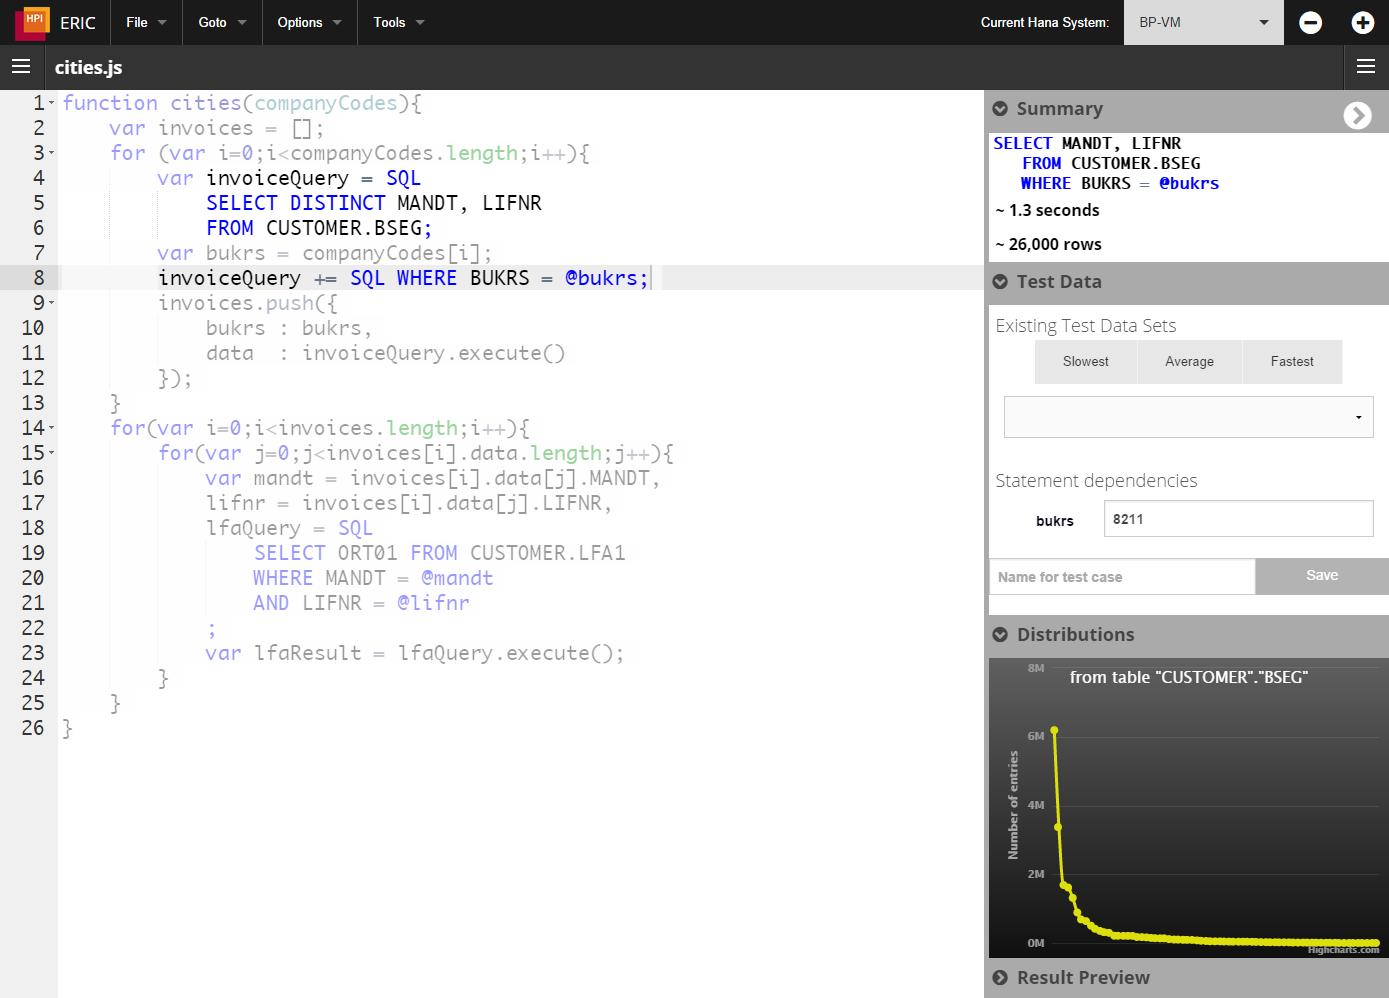
\includegraphics[width=0.95\textwidth]{figures/ide.png}
	\caption{Screenshot der Web-IDE »ERIC«}
	\label{fig:ide}
\end{figure}

Die im Rahmen des Bachelorprojektes ``Modern Computer-Aided Software Engineering'' entwickelte Web-IDE namens »ERIC« (Abbildung \ref{fig:ide}) vereint eine Reihe von Konzepten zur Entwicklung von Geschäftsanwendungen mit dem Fokus auf der besseren Integration von Informationen aus Datenbanken.
Besonders die Schärfung des Bewusstseins für Daten und Datenmengen sowie das vorausschauende Entwickeln in Hinblick auf die Skalierung der Anwendung soll gefördert werden.
Grundlage dafür bietet die Einbettung von SQL in die Programmiersprache der Geschäftsanwendung \cite{Horschig2014} (mehr Details dazu in Kapitel \ref{sec:dependencydetection}).
Durch das Parsen des Quellcodes \cite{Horschig2014} und der darin enthaltenen SQL-Statements \cite{Schulz2014} werden die Voraussetzungen geschaffen, Analysen und Visualisierungen der Datenabfragen durchzuführen.
Unter anderem kann anschließend eine Abschätzung über die Laufzeiten und Ergebnisgrößen von SQL-Statements gegeben werden, sowie eine Vorschau der Ergebnisse und die Verteilung der Daten in den angefragten Spalten.
Für die Berechnung der abgeschätzten Laufzeiten und Ergebnisgrößen stehen zwei Verfahren zur Auswahl: auf Basis von Sampling \cite{Exner2014} werden mithilfe von Teilmengen der Relationen ungefähre Größen hochgerechnet und durch den Ansatz des Machine Learnings \cite{Mues2014} können Ergebnisse vergangener Anfragen als Grundlage der Berechnung genutzt werden.

\begin{figure}[ht]
	\centering
  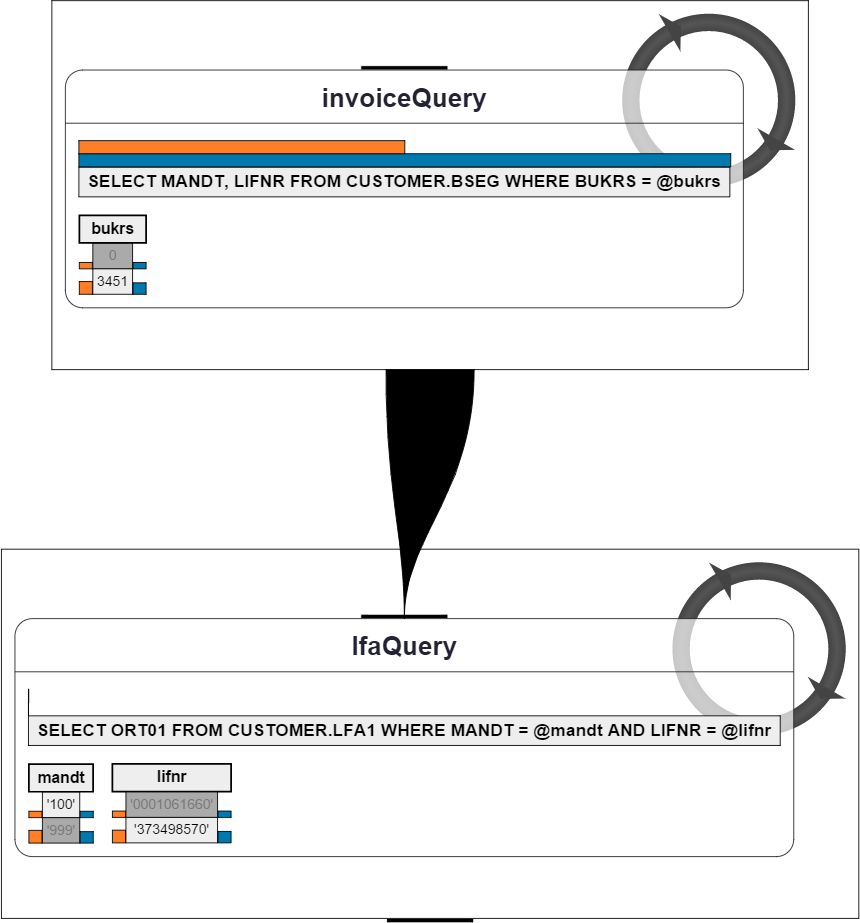
\includegraphics[width=0.7\textwidth]{figures/feedback.png}
	\caption{Visualisierung des Kontrollflusses}
	\label{fig:feedback}
\end{figure}

Zusätzlich ist es möglich den Verlauf des Kontrollflusses in Zusammenhang mit den Datenanfragen zu visualisieren \cite{Frahnow2014} (siehe Abbildung \ref{fig:feedback}) um die Ursachen von Performance-Problemen ausfindig zu machen.

Die betrachteten Features für die Analysen von SQL-Statements haben dabei zwei Voraussetzungen: das SQL-Statement muss komplett erfasst und dessen variable Parameter müssen testweise mit Werten belegt sein.

\begin{lstlisting}[caption={Variablen nehmen Einfluss auf die SQL-Query und -Parameter}, label={lst:ide}, language=JavaScript]
		var customer = request.body.customer,
		    negative = request.body.negative,
				filter = [],
		    stmt = "SELECT * FROM CUSTOMER.BSEG";
		if(negative){
			filter.push("BSEG.XNEGP = 'X'");
		}
		if(customer){
			filter.push("BSEG.KUNNR = '" + customer + "'");
		}
		if(filter.length > 0){
		stmt += " WHERE " +  filter.join(" and ");
\end{lstlisting}

Schon einfache Algorithmen, wie im Code-Beispiel \ref{lst:ide}, lassen das SQL-Statement auf Basis von Programmvariablen variieren (\texttt{negative}) und belegen die SQL-Parameter in Abhängigkeit von beispielsweise Sitzungsdaten, Formularen oder Anfrageparametern mit unterschiedlichen Werten (\texttt{customer}).
Dadurch ist es für den Entwickler schwer abzuschätzen, welche Testwerte repräsentativ sind oder sogar Randfälle darstellen und die Antwortzeit der Anwendung in die Höhe treiben.
Deshalb ist es wichtig, sinnvolle Testwerte und Kombinationen von Testwerten zu nutzen, die die verschiedenen Szenarien innerhalb der Anwendung abdecken.
Mit der Theorie und möglichen Algorithmen zum Vorschlagen dieser Daten beschäftigt sich diese Bachelorarbeit und diskutiert sie in den folgenden Kapiteln.

	\section{Verkn{\"u}pfung von SQL mit dem Anwendungskontext}\label{sec:dependencydetection}

%%%%%%%%%%%%%%%%
%
%    Verknüpfung von SQL mit dem Anwendungskontext
%
%%%%%%%%%%%%%%%%

Mit der Einbettung von SQL-Anfragen in andere Programmiersprachen, zum Beispiel in JavaScript\footnote{ECMAScript Language
Specification: \url{http://www.ecma-international.org/publications/files/ECMA-ST/Ecma-262.pdf}}, treffen zwei unterschiedliche Konzepte aufeinander: die imperative Programmiersprache der Anwendung und die deklarative Abfragesprache der Datenbank.

Häufig fließen dabei Informationen aus dem Kontext der Anwendung in das SQL-Statement ein, zum Beispiel als Parameter für Filterbedingungen.
Ebenso können sie sich durch die Steuerung des Kontrollflusses auf das Erstellen von SQL-Statements auswirken.
Im Folgenden werden deshalb die verschiedenen Varianten von SQL-Statements, deren Erstellung sowie Zusammenhänge mit Quellcodevariablen dargestellt.

\subsection{Dynamische Erstellung von SQL-Statements}
SQL-Statements können auf verschiedenste Weisen in den Quellcode einer Anwendung integriert werden, die sich vor allem durch die Stärke der Bindung von SQL-Statements und dem umliegenden Anwendungskontext unterscheiden.
Grundlegend kann man drei Arten differenzieren:

\subsubsection{Statische SQL-Statements}

	\begin{lstlisting}[caption={Statisches SQL-Statement eingebettet im Quellcode}, label={lst:staticsql}, language=JavaScript]
		var stmt = "SELECT *
		FROM CUSTOMER.BSEG LEFT OUTER JOIN CUSTOMER.LFA1
		ON BSEG.MANDT = LFA1.MANDT AND BSEG.LIFNR = LFA1.LIFNR";
		stmt.execute();
	\end{lstlisting}

Statische SQL-Statements bleiben über den Kontrollfluss hinweg unverändert und sind unabhängig vom umliegenden Kontext der Anwendung (siehe Code-Beispiel \ref{lst:staticsql}).
Sie können für Anfragen genutzt werden, die jederzeit dieselben Informationen aus der Datenbank auslesen (zum Beispiel das Auflisten aller Kunden).
Diese Datenbankanfragen sind für Analysen leicht aus dem Quellcode herauszuparsen und müssen nicht verändert oder mit Testwerten ergänzt werden.

\clearpage
\subsubsection{Prepared SQL-Statements}

	\begin{lstlisting}[caption={Prepared Statements eingebettet im Quellcode}, label={lst:preparedsql}, language=JavaScript]
		var stmt = con.prepareStatement("
		SELECT *
		FROM CUSTOMER.BSEG LEFT OUTER JOIN CUSTOMER.LFA1
		ON BSEG.MANDT = LFA1.MANDT AND BSEG.LIFNR = LFA1.LIFNR
		WHERE BSEG.KUNNR = ?");
		stmt.setInt(1, 23342341);
		stmt.execute();
	\end{lstlisting}

Der Anwendungsfall von Prepared Statements ist das mehrfache Ausführen derselben Anfrage mit verschiedenen Parameterwerten.
Dabei werden die variablen Stellen mit Fragezeichen versehen und vor der Datenabfrage explizit gesetzt.
Die im Code-Beispiel \ref{lst:preparedsql} gezeigte Variante setzt dabei in Zeile 6 einen konstanten Wert (23342341) für \texttt{BSEG.KUNNR} ein.
Häufig kommen diesen Informationen aus der Anfrage vom Nutzer oder Sitzungsdaten und sind damit nicht als Konstanten im Quellcode erfasst.
Das SQL-Statement ist somit abhängig von den zu setzenden Parameterwerten, wird jedoch nicht strukturell verändert.

\subsubsection{Dynamische SQL-Statements}

	\begin{lstlisting}[caption={Der Kontrollfluss verändert dynamische SQL-Statements}, label={lst:dynamicsql}, language=JavaScript]
		var customer = request.body.customer,
		    customerTo = request.body.customerTo,
		    stmt = "SELECT *
					FROM CUSTOMER.BSEG LEFT OUTER JOIN CUSTOMER.LFA1
					ON BSEG.MANDT = LFA1.MANDT AND BSEG.LIFNR = LFA1.LIFNR
					WHERE ";
		if(customer && !customerTo){
			stmt += "BSEG.KUNNR = '" + customer + "'";
		}
		if(customer && customerTo){
			stmt += "BSEG.KUNNR BETWEEN '" + customer +
							"' AND '" + customerTo + "'" ;
		}
	\end{lstlisting}

Dynamische SQL-Statements werden erst zur Laufzeit in Abhängigkeit vom Kontrollfluss des Programms erstellt.
So ist es möglich, Variablen aus der Anwendung sowohl zur Anpassung des SQL-Statements zu nutzen, als auch als Parameter für die Abfrage.
Es entsteht eine enge Bindung des Kontrollflusses an das resultierende SQL-Statement, wodurch die Variabilität steigt, aber auch mit zunehmender Komplexität das Lesen und Verstehen der Anwendung erschwert wird.
Im Code-Beispiel \ref{lst:dynamicsql} verändert sich das SQL-Statement durch das Setzen bzw. Nicht-Setzen von Anfrageparametern durch den Nutzer.
Dabei kann der Nutzer entscheiden, ob er die Informationen für eine konkrete Kundennummer (Zeile 5 bis 7) oder für ein Intervall von Kundennummern (Zeile 8 bis 11) abruft.
In beiden Fällen gibt es einen konstanten Part der Anfrage (Zeile 1 bis 4) und es fließen die Anfrageparameter in das SQL-Statement ein (\texttt{customer}, \texttt{customerTo}).

Im folgenden Abschnitt werden diese Beziehungen auf Basis von Variablen aus dem Kontext der Anwendung ausführlicher untersucht.


\subsection{Verkn{\"u}pfung von SQL-Parametern und Quellcodevariablen}\label{sec:sqlandsourcecode}
Aus dem Code-Beispiel \ref{lst:dynamicsql} geht bereits deutlich hervor, dass Kontextvariablen einen Einfluss auf das SQL-Statement und vorrangig dessen Parameter haben.
Allerdings wurden in den vorherigen Beispielen SQL-Teile stets nur als Zeichenketten in der Anwendung genutzt.
Durch diese Umwandlung verlieren sie ihre Komfortfunktionen (z.B. Autovervollständigung und Syntaxüberprüfung) und bergen zeitgleich das Risiko von Fehlern, zum Beispiel durch vergessene Leerzeichen, ohne die das finale SQL-Statement nicht valide wäre.
Um die Nachteile dieser Konkatenation von Zeichenketten abzuschaffen, kann der Quellcode in die Syntax nach Horschig \cite{Horschig2014} übertragen werden (vgl. Code-Beispiel \ref{lst:newsql}).
Durch die Einbettung der Datenbankanfragen nach dem Prinzip von Language Boxes \cite{diekmann2013parsing} werden die Konzepte von SQL und der umgebenen Sprache miteinander kombiniert und es entstehen Synergien, die die Entwicklung der Anwendung vereinfachen und den Quellcode leichter verständlich machen, zum Beispiel durch die explizite Verknüpfung von Quellcodevariablen mit SQL-Statements und -Parametern.

\clearpage
	\begin{lstlisting}[caption={Darstellung des Code-Beispiels \ref{lst:dynamicsql} in der Syntax nach \cite{Horschig2014}}, label={lst:newsql}, language=JavaScriptSQL]
		var customer = request.body.customer,
		    customerTo = request.body.customerTo,
		    stmt = SQL[CUSTOMER]
					SELECT *
					FROM BSEG LEFT OUTER JOIN LFA1
					ON BSEG.MANDT = LFA1.MANDT AND BSEG.LIFNR = LFA1.LIFNR;
		if(customer && !customerTo){
			stmt += SQL WHERE BSEG.KUNNR = @customer;
		}
		if(customer && customerTo){
			stmt += SQL WHERE BSEG.KUNNR BETWEEN @customer AND @customerTo;
		}
	\end{lstlisting}

Die einzelnen SQL-Blöcke im Code-Beispiel \ref{lst:newsql} beginnen mit einer \texttt{SQL}-Anweisung, auf die der eigentliche SQL-Text folgt und mit einem Semikolon abgeschlossen wird.
In Zeile 3 wird zusätzlich das Schema \texttt{CUSTOMER} für das Statement \texttt{stmt} festgelegt.
Markant dabei ist die Verwendung des Zeichens \texttt{@}.
Durch diese Anweisung wird der zum Zeitpunkt der Definition des SQL-Statements aktuelle Wert der Variable \texttt{customer} fest im SQL-Statement gesetzt.

Um eine Wiederverwendung von SQL-Blöcken zu ermöglichen, können sie ähnlich wie Funktionen als SQL-Templates \cite{Horschig2014} formuliert werden.

	\begin{lstlisting}[caption={SQL-Templates ermöglichen Wiederverwendung}, label={lst:sqlfunctions}, language=JavaScriptSQL]
	var toleranceDays = request.body.toleranceDays,
	    percentageRate = request.body.percentageRate,
	    getFunctionParameters = SQL[CUSTOMER](xskr1)
				REGUP.BUDAT, REGUP.WSKTO, REGUP.BLDAT,
				:xskr1, @toleranceDays, @percentageRate;
	getFunctionParameters(11).execute();
	\end{lstlisting}

Neben dem \texttt{@} kann so zusätzlich \texttt{:} zur Referenzierung dienen.
Der Unterschied liegt darin, dass der Wert des Parameters (\texttt{xskr1}) erst beim Aufruf des SQL-Templates festgesetzt wird, die Werte von \texttt{toleranceDays} und \texttt{percentageRate} hingegen zum Zeitpunkt der Definition des SQL-Statements.
Das SQL-Template \texttt{getFunctionParameters} kann anschließend mittels der Anweisung \texttt{+=} einem existieren SQL-Statement angefügt werden.

Eine solche Wiederverwendung ist z.B. nützlich bei SQL-Statements, die in einer Schleife verwendet werden und ein oder mehr variable Bestandteile haben.
In diesem Fall wird die Anfrage nur einmal als SQL-Template definiert und kann innerhalb der Schleife mit den entsprechenden Parameterwerten aufgerufen werden.

An diesen Code-Beispielen wird deutlich, dass Variablen häufig ein SQL-Statement verändern und in dieses an verschiedenen Stellen einfließen.
Im Folgenden wird deshalb eine Unterscheidung der Variablenverbindung zwischen dem eingebetteten SQL und dem umliegende Quellcode vorgenommen.

\nomenclature{ERP}{Enterprise Resource Planning}
\subsection{Differenzierung von Kontrollfluss- und SQL-Statement-Abhängigkeiten}\label{sec:controlflowandsqldependencies}
Neben dem direkten Einfließen von Variablen in ein SQL-Statement (vgl. Kapitel \ref{sec:sqlandsourcecode}), können diese auch (nur) als Abhängigkeit im Kontrollfluss auftreten.

	\begin{lstlisting}[caption={Verschiedene Arten der Abhängigkeit von Variablen}, label={lst:differentdep}, language=JavaScriptSQL]
		var noDunning = request.body.noDunning,
		    customer = request.body.customer,
		    selection = request.body.selection;
		var stmt = SQL[CUSTOMER]
			SELECT @selection
			FROM BSEG LEFT OUTER JOIN LFA1
			ON BSEG.MANDT = LFA1.MANDT AND BSEG.LIFNR = LFA1.LIFNR;
		if(noDunning){
			stmt += SQL WHERE BSEG.MANST = 0;
		}
		if(customer){
			stmt += SQL WHERE BSEG.KUNNR = @customer;
		}
	\end{lstlisting}

Im Code-Beispiel \ref{lst:differentdep} sind alle drei Möglichkeiten der Einflussnahme auf SQL-Statements durch Variablen dargestellt.
Sie können direkt in das SQL-Statement eingebunden werden (\texttt{selection}), das SQL-Statement in der Struktur manipulieren (\texttt{noDunning}) oder beides zugleich vornehmen (\texttt{customer}).

Schon bei diesen einfachen Algorithmen ist es für Entwickler schwer, relevante Testwerte zu finden, um Analysen des resultierenden SQL-Statements zu ermöglichen, ohne z.B. die Inhalte der Relationen der zugrundeliegenden Datenbank zu kennen.
Zudem können die Relationen kryptische Werte in unverständlich benannten Spalten enthalten.
Beispielsweise bedeutet in einem SAP ERP-System der Eintrag \texttt{R} in der Spalte \texttt{BSEG.ZLSCH}, dass eine Rechnung mittels Euroüberweisung beglichen wurde.

Zusätzlich stellt die Variation an Verknüpfungen von Variablen und SQL-Statements eine Herausforderung für das Vorschlagen passender Testdaten dar, denn nicht immer können Informationen aus der Datenbank genutzt werden.
Aus diesem Grund werden in Kapitel \ref{chap:testdatasuggestions} verschiedene Lösungsstrategien und Ansätze erörtert, die den Entwickler unterstützen, repräsentative Testwerte durch passende Vorschläge zu finden, um aussagekräftige Analysen auf SQL-Statements zu ermöglichen.

	\section{Generierung von Vorschlägen für Variablen-Belegungen}\label{chap:testdatasuggestions}

%%%%%%%%%%%%%%%%
%
%   Automatische Vorschlagsgenerierung für Variablen-Belegungen
%
%%%%%%%%%%%%%%%%

%- FOKUS darauf!
%- ein gesamttestfall für kompletten algorithmus? --> Clemens
%- Testfällt updatebar machen

Um dem Entwickler repräsentative Testwerte, die die Variationspunkte eines SQL-Statements beeinflussen, vorzuschlagen, gibt es verschiedene Strategien.
Grundlage dafür bietet, wie anfangs erwähnt, ein Datenbanksystem mit den enthaltenen Echt-Daten.
In den folgenden Beispielen werden Unternehmensdaten aus einer SAP-Infrastruktur einer Aktiengesellschaft genutzt.
Die Integration solcher Datenbanksysteme und die Administration von den genutzten Test-Daten werden im Kapitel \ref{chap:testdataadministration} näher erläutert.

Neben der Betrachtung der Charakteristiken von Daten innerhalb der Datenbank, ist vor allem die Verknüpfung mit Analyse-Ergebnissen, vorrangig den Laufzeit-Messungen, ein Kriterium für die Generierung der Vorschläge.
Mittels Auswahl unterschiedlicher, vorgeschlagener Testwerte ist es dem Entwickler möglich konkrete Ausprägungen von SQL-Statements nachzuvollziehen und durch die Auswertung der Messungen gegebenenfalls Optimierungen durchzuführen bis das gewünschte Performance-Verhalten erreicht ist.


\subsection{Vorschläge auf Basis von Daten-Charakteristiken}\label{chap:datacharacteristics}
Der erste Anhaltspunkt für das Vorschlagen relevanter Testwerte ist die Charakteristik der Datenbankinhalte.
Primär spielen dabei die Verteilung der Daten innerhalb der Relationen und die Anzahl ihrer unterschiedlichen Ausprägungen eine Rolle.

%\begin{figure}
%\centering
	%\begin{tikzpicture}
		%\begin{axis}[
				%axis lines=left,
				%width  = 0.85*\textwidth,
				%height  = 6cm,
				%symbolic x coords={Males,Females},
				%xtick=data,
				%enlarge x limits=0.5,
				%bar width=40pt,
				%ybar,
				%ylabel={Percentage},
				%ymin=0.0,
				%ymax=100.0,
				%]
				%\addplot[ybar,fill=light-gray] coordinates {
						%(Males,55)
						%(Females,45)
				%};
		%\end{axis}
	%\end{tikzpicture}
	%\caption{(TODO: ersetzten durch statistik in BSEG.) Verteilung der Werte in der Spalte Gender.}
	%\label{fig:gender}
%\end{figure}

\pgfkeys{
    /pgf/number format/precision=0,
    /pgf/number format/fixed zerofill=true,
    /pgf/number format/fixed,
		/pgf/number format/.cd,
		use comma,
		1000 sep={.}
}

\begin{figure}
\centering
	\begin{tikzpicture}
		\begin{axis}[
			axis lines=left,
			xbar, xmin=0,
			width=0.85*\textwidth,
			height=6cm,
			enlarge y limits=0.1,
			xlabel={Absolute Anzahl distinkter Werte},
			symbolic y coords={MANDT,GJAHR,ZLSCH,BUKRS,AUGDT,LIFNR,SKFBT,KUNNR,WRBTR,BELNR},
			ytick=data,
			bar width=5pt,
			nodes near coords, nodes near coords align={horizontal},
			]
			\addplot[fill=light-gray] coordinates {
				(5636590,BELNR)
				(560628,WRBTR)
				(408015,KUNNR)
				(228722,SKFBT)
				(48407,LIFNR)
				(2304,AUGDT)
				(71,BUKRS)
				(31,ZLSCH)
				(10,GJAHR)
				(2,MANDT)
			};
		\end{axis}
	\end{tikzpicture}
	\caption{Verteilung distinkter Werten einer Auswahl von Spalten aus BSEG}
	\label{fig:bseg}
\end{figure}

Die Abbildung \ref{fig:bseg} zeigt eine Auswahl der 326 Spalten der BSEG-Tabelle aus einem SAP-System.
Die Tabelle enthält alle einzelnen Belegpositionen zu den Buchungsbelegen des Unternehmens.
Eine Erläuterung zu der Bedeutung der einzelnen Spalten befindet sich im Anhang (Tabelle \ref{tab:bsegerlaeuterung}).

Sollte die Anzahl der distinkten Werte einstellig sein (beispielsweise bei der Spalte MANDT), können dem Entwickler alle möglichen Ausprägungen in einem Auswahl-Menü zur Verfügung gestellt werden.
Damit wird gleichzeitig auch sichergestellt, dass nur Werte eingegeben werden können, die beim testweisen Ausführen des SQL-Statements ein Ergebnis zurückgeben.
Auf der anderen Seite können sich Spalten jedoch über eine große Menge von verschiedenen Datenausprägungen erstrecken, wie zum Beispiel bei Belegnummern (BELNR), was eine einfache Auswahl passender Testdaten kompliziert gestaltet.
Für diesen Fall werden Äquivalenzklassen anhand der Vorkommen der Werte erzeugt, die sich unterteilen in: die drei häufigste Werte, die drei seltensten Werte, drei Werte um den Median und der Rest.

Für die häufigsten Werte wird eine aufsteigende Sortierung der Anzahl des Vorkommens eines Wertes vorgenommen und die ersten drei selektiert.
Sollten mehrere Werte dieselbe Anzahl an Vorkommen vorweisen, werden sie zusätzlich anhand ihrer Werte aufsteigend sortiert.
Im Unterschied dazu wird bei der Klasse der seltensten Werten eine absteigende Sortierung vorgenommen.
Für die Werte um den Median muss zuerst die Anzahl der verschiedene Werte ermittelt werden.
Anschließend dient die Halbierung des Ergebnisses als Offset für die Bestimmung der drei Werte.
Die SQL-Statements dazu befinden sich im Anhang als Code-Beispiel \ref{lst:distinctvalues}.

Dieser Ansatz ist zum Vorschlagen einzelner Testwerte nützlich, stößt jedoch an seine Grenzen, sobald mehrere Parameter genutzt werden und diese voneinander abhängig sind.
Im Code-Beispiel \ref{lst:dynamicsql} aus dem Kapitel \ref{sec:dependencydetection} werden beispielsweise offene Rechnungen und deren Einzelposten gesucht.
Die Variable \texttt{customer} gibt dabei die Kundennummer an, mit der die Rechnungen assoziiert sind.
Sucht man nun nach der Kundennummer mit den meisten Rechnungen, bedeutet dies nicht zwangsläufig, dass man auch die mit den meisten Einzelposten oder höchsten Gesamtsummen findet.
Diese, noch recht einfache, Abhängigkeit kann beliebig erweitert werden.
Damit entstehen komplexe SQL- und Programm-Strukturen, die durch das einfache Vorschlagen anhand von Charakteristiken einzelner Spalten nicht zwangsläufig die Randfälle aufzeigen, die der Entwickler sucht.
Aus diesem Grund ist die Betrachtung von Messwerten der Analyse-Ergebnisse eine sinnvolle Erweiterung um die Genauigkeit der Vorschläge zu steigern.

\subsection{Adaptive Vorschlagsgenerierung durch Laufzeit-Analysen}\label{chap:adaptive}
Laufzeit-Analysen (\cite{Exner2014}, \cite{Mues2014}) ermöglichen das Verhalten von Datenbankzugriffen in Geschäftsanwendungen nachzuvollziehen.
Die variablen Stellen von SQL-Statements werden dabei durch die vom Entwickler ausgewählten Werte gefüllt.
Im nächsten Schritt werden nun diese atomaren Vorschläge kombiniert und mit dem dazugehörigen Ergebnis aus der Laufzeit-Analyse verknüpft.
Dies ermöglicht Vergleichbarkeit verschiedener Konstellationen.
Für die Erstellung der initialen Daten können zwei verschiedene Ansätze verfolgt werden.

Mithilfe der Brute-Force-Methode können alle Kombinationen durchprobiert und gemessen werden.
Der enorme Aufwand, gerade bei besonders Relationen mit vielen Einträgen und distinkten Werten in den Spalten, stellt jedoch aufgrund der enormen Berechnungszeit ein großes Hindernis dar.

Dem gegenüber steht der adaptive Ansatz, bei dem der Testdaten-Bestand kontinuierlich erweitert wird.
Diese Variante speichert die Ergebnisse der Laufzeit-Analysen mit den dazugehören Testdaten-Konstellationen als Testdaten-Sets.
Sobald mehrere dieser Sets vorhanden sind, können dem Entwickler drei Vorauswahl-Optionen gegeben: das Testdaten-Set mit der höchsten Laufzeit, mit der geringsten Laufzeit und mittlerer Laufzeit.

Um für diese Methode eine Datengrundlage zu schaffen, werden die in Kapitel \ref{chap:datacharacteristics} ermittelten Werte genutzt um initiale Kombinationen zu bilden und ihre Laufzeiten zu berechnen.
Durch Eingabe weiterer Werte durch den Entwickler kann anschließend das Datenmodell kontinuierlich erweitert und zunehmend verbessert werden, zu sehen im Code-Beispiel \ref{lst:developerinput}.

\begin{lstlisting}[caption={Eingaben von Testwert-Konstellationen erweitern gegebenenfalls das Datenmodell}, label={lst:developerinput}, language=Python]
	hier
	kommt
	der
	algorithmus
	rein
\end{lstlisting}

TODO: Algorithmus beschreiben.

\subsection{Betrachtung von Zeitbereichsanfragen}
Ein typischer Bestandteil von Datenbankanfragen in Geschäftsanwendungen sind Bereichsfilter mittels \texttt{column BETWEEN x AND y},  insbesondere für Zeiträume.
Der in Kapitel \ref{chap:datacharacteristics} vorgestellte Algorithmus generiert Vorschläge basierend auf binären Operationen (zumeist Vergleiche), wohingegen ein Bereichsfilter ternär ist.
Deshalb ist eine besondere Betrachtung für passende Vorschläge sinnvoll.

Sollte eine Bereichsanfrage erkannt werden, die eine Spalte vom Datentyp \texttt{DATE} referenziert, so kann der Entwickler eine vorgeschlagene Zeitraumgröße (z.B. eine Woche, ein Monat oder ein Jahr) auswählen oder selbst festlegen.
Anschließend wird die referenzierte Spalte mithilfe der angegebenen Zeitraumgröße gescannt, ähnlich dem Prinzip des Sliding Window\footnote{\url{http://en.wikipedia.org/wiki/Sliding_window_protocol}}.
Auf dieser Basis werden, ähnlich dem Algorithmus aus Kapitel \ref{chap:datacharacteristics}, bis zu 3 Vorschläge für die größte, kleinste und mittlere Anzahl an Resultaten erzeugt.
Alternativ steht es dem Entwickler offen, Start- und Enddatum eigenständig festzulegen.

\subsection{Integration in die IDE}
\begin{figure}[ht]
	\centering
  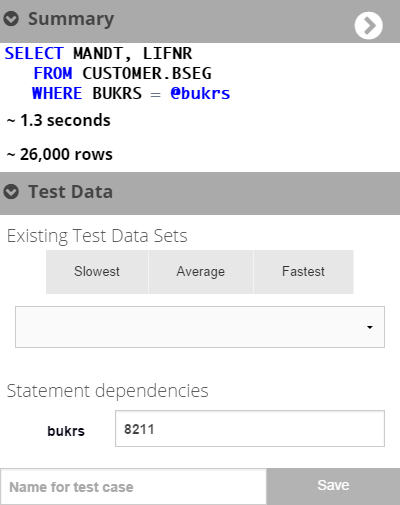
\includegraphics[width=0.4\textwidth]{figures/integration.png}
	\caption{Einbindung der Vorschläge in die Sidebar der Web-IDE}
	\label{fig:ideintegration}
\end{figure}

Die in Kapitel \ref{chap:datacharacteristics} und \ref{chap:adaptive} erzeugten Vorschläge werden in der zur Web-IDE gehörenden Datenbank gespeichert und in einer Sidebar im Frontend eingebunden (vgl. Abbildung \ref{fig:ideintegration}).
Durch das Auswählen des Entwicklers einer Quelltext-Zeile mit SQL-Inhalt, werden die Informationen zu dem dazugehörigen SQL-Statement aggregiert und aufbereitet (vgl. Kapitel \ref{chap:entwicklungsumgebung}) und schließlich in der Sidebar angezeigt.

TODO: Betrachtung vom AST?

Aus der im Kapitel \ref{chap:adaptive} ermittelten Menge an Testdaten-Sets werden zum einen die drei mit der höchsten, geringsten und durchschnittlichen Laufzeit angeboten, zum anderen ein Auswahl-Menü mit allen gespeicherten Sets.
Die Auswahl einer dieser Optionen füllt die Eingabefelder für die Testdaten automatisch mit den gespeicherten Werten und löst eine Analyse aus.
Möchte der Entwickler weitere Testdaten-Sets hinzufügen, so kann er diese benennen und direkt abspeichern.
Die Verwaltung dieser gespeicherten Daten wird im folgenden Kapitel behandelt.

\subsubsection{Nutzung von Meta-Informationen für UI-Elemente}
Um den Entwickler bei der Eingabe von Testdaten zu unterstützen, können Meta-Informationen über die Relationen genutzt werden.
Dazu kann der Datentyp von Spalten einer Relation für die Erstellung der Eingabefelder genutzt werden kann.
Beispielweise kann die Eingabe, die eine Spalte mit Datumsangaben referenziert, durch einen Kalender vereinfacht werden.
Auch die Einschränkung auf Datentypen, z.B. Ganzzahlen, kann fehlerhafte Eingabe durch den Entwickler verhindern.
Eine weitere Unterstützung ist die Autovervollständigung von teilweise eingegeben Werten.
Mittels des SQL-Operators \texttt{LIKE} kann dafür nach Daten gesucht werden, die dem Muster der bisherigen Eingabe entsprechen.
	\section{Verwaltung von Test-Daten und Test-Systemen}\label{chap:testdataadministration}

%%%%%%%%%%%%%%%%
%
%    Verwaltung von Test-Daten und Test-Systemen
%
%%%%%%%%%%%%%%%%

An das Backend der Web-IDE ist eine eigene SAP Hana-Instanz angebunden.
Darin werden die Testdaten-Sets und Zugangsdaten für Test-Systeme hinterlegt.
Im folgenden geht es um das zugrundeliegende Schema, die Integration verschiedener Test-Systeme und das Pflegen der Test-Daten, insbesondere in Hinblick auf deren Gültigkeit.

\subsection{Datenschema für Testdaten-Sets}
Die Herausforderung beim Speichern der Testdaten-Sets liegt in der Wiederzuordnung zu den Variablen in der vom Entwickler geöffneten Quelltext-Datei.
Der in der Web-IDE genutzte Quelltext-Parser \cite{Horschig2014} nutzt symbolische Ausführung \cite{DBLP:journals/cacm/King76} zur Bestimmung von Variablen und deren eventuell bereits festgelegten Werten.
Die auf diesem Wege gefundenen Variablen bekommen eine eindeutige Kennzeichnung, die zum Identifizieren genutzt werden kann.
Sollten sie im Laufe des Programmflusses in mindestens ein SQL-Statement einfließen, werden sie als Test-Variablen betrachtet.
Eine Menge von Test-Variablen bildet zusammen mit dem Dateipfad und einem vom Entwickler angegebenen Namen ein Test-Set.
Diese Test-Sets können wiederum in Beziehung mit dem Test-System gebracht werden, auf dem die Performance-Analysen erfolgten, um die Abhängigkeit der System-Auswahl auf die Laufzeiten der Test-Sets zu berücksichtigen.
In Abbildung \ref{fig:erm} ist das dazugehörige Datenschema dargestellt.

\newcommand {\key}[1]{\underline{#1}}

\begin{figure}[ht]
	\centering
	\begin{tikzpicture}[node distance = 7em]
		\node [entity] (testset) {Test Set};
		\node [attribute] (tsid) [left of=testset] {\key{ID}} edge (testset);
		\node [attribute] (tsname) [above right of=testset] {Name} edge (testset);
		\node [attribute] (tsfilepath) [above left of=testset] {File Path} edge (testset);
		\node [relationship] (tshastv) [right of=testset] {has} edge (testset);
		\node [entity] (testvalue) [right of=tshastv] {Test Variable} edge [total] (tshastv);
		\node [attribute] (tvid) [above left of=testvalue] {\key{ID}} edge (testvalue);
		\node [attribute] (tvvariable) [above right of=testvalue] {Variable} edge (testvalue);
		\node [attribute] (tvvalue) [right of=testvalue] {Value} edge (testvalue);
		\node [relationship] (tshastsys) [below = 0.5cm of testset] {has} edge (testset);
		\node [entity] (testsystem) [below = 0.5cm of tshastsys] {Test System} edge [total] (tshastsys);
		\node [attribute] (tsysname) [left of=testsystem] {\key{Name}} edge (testsystem);
		\node [attribute] (tsyshost) [below right of=testsystem] {Host} edge (testsystem);
		\node [attribute] (tsysport) [below of=testsystem] {Port} edge (testsystem);
		\node [attribute] (tsysuser) [below left of=testsystem] {User} edge (testsystem);
		\node [attribute] (tsyspassword) [right = 0.5cm of testsystem] {Password} edge (testsystem);
	\end{tikzpicture}
	\caption{ER-Diagram für die Administration von Test-Sets und -Systemen}
	\label{fig:erm}
\end{figure}

\subsection{Caching und Gültigkeit von Test-Daten}
Um nicht für jede Vorschlagsanfrage einen Datenbankzugriff durchzuführen, werden die Testdaten und Testdaten-Sets sowohl im Frontend als auch im Backend gecached.
Die Caches unterscheiden sich in der Hinsicht, dass es einen Frontend-Cache für jede Sitzung eines Entwicklers gibt, wohingegen der Backend-Cache global agiert.
Eine Anfrage für Testdaten-Vorschläge zu einer Spalte einer Relation wird dabei erst versucht durch den Frontend-Cache zu beantworten.
Sollten dort keine passenden Daten vorliegen, wird eine Anfrage an das Backend ausgelöst.
Dort versucht der Backend-Cache als erste Instanz diese Anfrage zu beantworten.
Sollten auch dort keine Daten vorliegen, werden die Vorschläge mithilfe der in Kapitel \ref{chap:testdatasuggestions} vorgestellten Algorithmen bestimmt und in den Caches hinterlegt.

Eine Herausforderung stellt das Überprüfen der Gültigkeit der Vorschläge und Testdaten-Sets dar.
Diese kann durch zwei Fälle beeinflusst werden: die Daten in der genutzten Datenbank werden verändert (erweitert, aktualisiert oder gelöscht) oder der Quelltext der Anwendung wird in einer Weise abgeändert, die die Variablen aus den SQL-Statements beeinflusst.

Für Ersteres gibt es Ansätze \cite{DBLP:conf/dasfaa/HarangsriSN97}, die kontinuierlich verändernde SQL-Statements nachverfolgen und dementsprechend ihren Algorithmus durch manuelles Hoch- bzw. Runterzählen der Anzahl von Einträgen in der betrachteten Relation anpassen.
Ein solches Vorgehen ist für die in Kapitel \ref{chap:testdatasuggestions} beschrieben Algorithmen nicht umsetzbar, da sie fest gekoppelt sind an die Werte in der Datenbank und nicht nur an ihre Anzahl.
Nichtsdestotrotz floss die Idee der Betrachtung von manipulierenden SQL-Statements mit in die Implementierung ein, indem ein Schwellwert für Datenveränderungen festgelegt wird (derzeit 10), ab dem eine Neubestimmung von Vorschlägen und initial berechneten Testdaten-Sets erfolgt.

Die Invalidierung der Daten durch Veränderung des dazugehörigen Quelltextes wurde im Zuge dieser Arbeit nicht betrachtet, ist aber als Weiterentwicklung geplant.
Die Schwierigkeit liegt darin, eine Granularität zu finden, auf der Änderungen zur Invalidierung führen, und gegebenenfalls diese Veränderung nachzuvollziehen.
Legt man die Granularitätsstufe auf das gesamte Dokument fest, würde dies dazu führen, dass die Test-Daten zu häufig als ungültig gekennzeichnet werden, obwohl das nicht zwangsläufig zutreffen muss.
Wählt man eine feine Granularitätsstufe (zum Beispiel alle Änderungen, die nur Variablen betreffen, die in SQL-Statements einfließen), so ist eine komplexe Nachverfolgung der Änderungen am Dokument über dessen verschiedene Revisionen notwendig.
Sollte ein Versionsverwaltungssystem für die Quelltext-Dateien genutzt werden, können dessen Informationen in er Nachverfolgung berücksichtig werden.

\subsection{Integration mehrerer Test-Systeme}
Typischerweise dient nicht nur ein System als Grundlage für Performance-Analysen einer Geschäftsanwendung, sondern ein Auswahl an Systemen mit unterschiedlichen Ausstattungsmerkmalen.
Dies kann mehrere Gründe haben.
In Hinblick auf die Daten können so Datenschutz-Bestimmungen eingehalten oder auch Datensätze mit verschiedene Charakteristiken getestet werden.
Zum anderen kann so auch die Auswirkung verschiedener System-Konfigurationen auf die Performance der Anwendung geprüft werden, wodurch Kosten gespart werden können, indem man eine passendes System für den Produktiveinsatz auswählt.
Realisiert wird dies durch ein Menü in der Web-IDE (vgl. Abbildung \ref{fig:hanainstances}) bei dem das gewünschte Test-System ausgewählt oder aber auch neue hinzufügt oder existierende entfernt werden können.
Die Zugangsdaten für die Systeme werden in der Datenbank der Web-IDE hinterlegt (vgl. Abbildung \ref{fig:erm}) und das derzeit vom Entwickler ausgewählte System in seinen Sitzungsdaten hinterlegt.
\begin{figure}[ht]
	\centering
  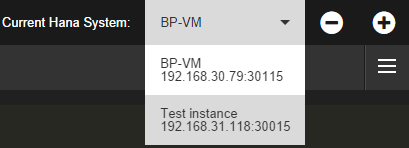
\includegraphics[width=0.6\textwidth]{figures/hana-instances.png}
	\caption{Auswahl-Menü für verschiedene Datenbank-Server}
	\label{fig:hanainstances}
\end{figure}


	\section{Fallbeispiel: Der Zahllauf}\label{chap:paymentrun}

\nomenclature{IT}{Information Technology}
Im Bereich der Geschäftsanwendungen gibt es eine Reihe hochkomplexer Prozesse, die in der IT abgebildet werden.
Einer davon ist der sogenannte Zahllauf, bei dem sich der Anwender eine Liste von offenen Zahlungen erst vorschlagen lässt, den Vorschlag überprüft und anschließend die Bearbeitung durch das System veranlasst.
Dabei spielen insbesondere die Abhängigkeiten von Zahlungen, Lieferanten und Rabattverträgen eine wichtige Rolle, da sie im Idealfall in eine günstige Konstellation für das Unternehmen resultieren und dadurch Einsparungen bei den Ausgaben ermöglichen.

Aus diesem Grund hat die Implementierung des dazugehörigen Algorithmus viele Einflussfaktoren. 
Zusätzlich erschweren große Relationen mit stark abgekürzten Namen von Feldern und Werten, die als Eingabe, Zwischenspeicher und Ausgabe dienen, das Erstellen einer daten- und performancebewussten Umsetzung.
Dies gilt besonders für domänenfremde Entwickler.
Umso wichtiger ist es, bereits frühzeitig in der Entwicklung relevante Testdaten zu nutzen, die auch Randfälle der Implementierung abdecken und Engpässe aufzeigen.
Dabei unterstützt die im Rahmen des Bachelorprojektes erstellte Web-IDE den Entwickler durch die in dieser Arbeit vorgestellten Ansätze zur Generierung von Testdatenvorschlägen.

In diesem Kapitel wird folgend exemplarisch die Implementierung des Zahllauf-Algorithmus mithilfe der Web-IDE vorgestellt.
Dabei steht die von Nutzereingaben geprägte Verarbeitung der Suche nach Belegen im Fokus.
Anschließend werden die vorgestellten Ansätze zur Testwertgenerierung anhand der Umsetzung des Fallbeispiels evaluiert.

\subsection{Implementierung des Algorithmus in der Web-IDE}

\begin{figure}[ht]
	\centering
  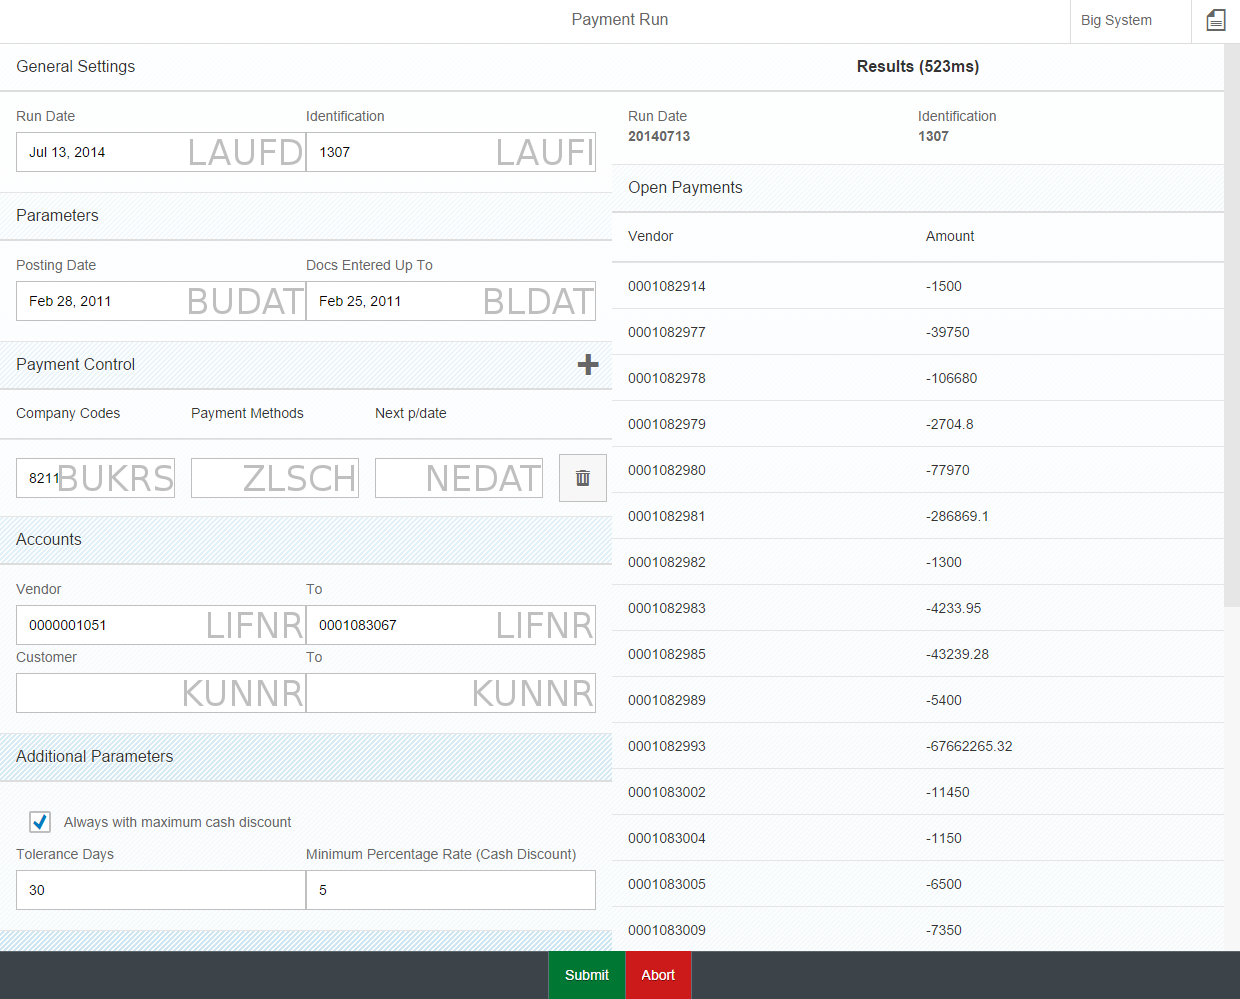
\includegraphics[width=1\textwidth]{figures/paymentrun.png}
	\caption{Eingabemaske des Zahllaufs}
	\label{fig:paymentrun}
\end{figure}

\nomenclature{UI}{User Interface}
Die in Abbildung \ref{fig:paymentrun} dargestellte Filtereingabemaske des Zahllaufs hat zwei Bestandteile. 
Zum einen können allgemeine Parameter für die Suche festgelegt werden (z.B. das Ausführungsdatum (Run Date) und der Bereich der Lieferantennummern (Vendor)).
Zum anderen dient die Eingabe in Form einer Tabelle (Payment Control) zur Festlegung von zusammenhängende Suchkriterien.
Jede Zeile der Tabelle besteht aus einem Filter nach Buchungskreis (Company Codes), Zahlmethoden (Payment Methods) und dem nächsten Ausführungsdatum (Next p/date) und entspricht damit einem eigenen Suchlauf.

Für die Implementierung des Frontends wurde das UI-Framework OpenUI5\footnote{\url{http://sap.github.io/openui5/}} von SAP genutzt.
Der Fokus dieses Kapitels liegt jedoch auf der Backendimplementierung auf Basis der SAP XS-Engine\footnote{\url{http://help.sap.com/hana/SAP_HANA_XS_JavaScript_Reference_en/index.html}}.

Der Algorithmus des Zahllaufs besteht aus 5 Schritten:
   \begin{enumerate}
      \item Parsen der JSON-Anfrage vom Frontend
			\item Selektion von Belegpositionen und Speicherung in der REGUP-Relation
			\item Berechnung von Zahldatum und Skonto
			\item Speicherung der Beleginformationen in der REGUH-Relation
			\item Senden einer JSON-Antwort
   \end{enumerate}

Die REGUP- und REGUH-Relationen dienen als datenbankinterne Zwischenspeicher für die ermittelten Ergebnisse.
Zur Selektion wird die Relation BSIK als materialisierte Sicht auf die BSEG-Relation genutzt.

Die Eingaben des Nutzers in der Filtermaske wirken sich insbesondere auf die Selektion der Belegpositionen aus.
Sie werden im ersten Schritt aus der JSON-Anfrage geparst (siehe Code-Beispiel \ref{lst:jsoninput} im Anhang) und fließen im Programmverlauf in das allgemeine SQL-Statement zur Selektion (siehe Code-Beispiel \ref{lst:regupgeneral} im Anhang) ein.

Code-Beispiel \ref{lst:laufi} zeigt exemplarisch wie die Projektion des SQL-Statements um das Ausführungsdatum (\texttt{LAUFD}) ergänzt wird.
Für das Identifikationsmerkmal (\texttt{LAUFI}) wird analog verfahren.

\begin{lstlisting}[caption={Ergänzung der Projektion um das Ausführungsdatum}, label={lst:laufi}, language=JavaScriptSQL]
	if(runDate){
			insertRegup += SQL SELECT @runDate as LAUFD;
	} else {
			insertRegup += SQL SELECT '' as LAUFD;
	}
\end{lstlisting}

Anschließend werden dem SQL-Statement das Buchungs- (\texttt{BUDAT}) und Erfassungsdatum (\texttt{BLDAT}) optional als Filter hinzugefügt (Code-Beispiel \ref{lst:budat}).

\begin{lstlisting}[caption={Einfügen zusätzlicher Filter}, label={lst:budat}, language=JavaScriptSQL]
	if(postingDate){
			insertRegup += SQL WHERE AND BSIK.BUDAT = @postingDate;
	}
	if(docsEnteredDate){
			insertRegup += SQL WHERE AND BSIK.BLDAT <= @docsEnteredDate;
	}
\end{lstlisting}

Für die Eingabe einer bzw. mehrerer Kundennummern (\texttt{KUNNR}) wird das bereits bekannte Code-Beispiel \ref{lst:newsql} aus Kapitel \ref{sec:sqlandsourcecode} genutzt und kann in leicht abgewandelter Form auch für Lieferantennummern (\texttt{LIFNR}) verwendet werden (Code-Beispiel \ref{lst:vendor}).

\begin{lstlisting}[caption={Unterscheidung zwischen Einzel- und Bereichsfilter}, label={lst:vendor}, language=JavaScriptSQL]
	if(vendor && !vendorTo ){
			insertRegup += SQL WHERE AND BSIK.LIFNR = @vendor;
	}
	if(vendor && vendorTo ){
			insertRegup += SQL WHERE AND BSIK.LIFNR BETWEEN @vendor
				AND @vendorTo;
	}
\end{lstlisting}

Das komplexeste Konstrukt der Eingabemaske ist die Tabelle für Kriterien zur Suche anhand von Buchungskreisen (\texttt{BUKRS}), Zahlmethoden (\texttt{ZLSCH}) und dem nächsten Ausführungsdatums (\texttt{NEDAT}) des Zahllaufs.
Die einzelnen Zellen einer Zeile bilden eine Konjunktion, wobei die Reihen untereinander jeweils disjunkt sind.
Die Komplexität entsteht durch die vielen Variationsmöglichkeiten der Eingabe.
So können Buchungskreise z.B. kommasepariert, mittels Klammern als Bereich oder beides kombiniert angegeben werden.
Die Zahlmethoden werden mit Großbuchstaben abgekürzt und aneinander gereiht um die Angabe mehrerer Methoden zuzulassen.

Die Verarbeitung der Nutzereingaben aus der Tabelle erfolgt dazu zeilenweise (siehe Code-Beispiel \ref{lst:paymentcontrol}).
Im ersten Schritt wird die Angabe der Buchungskreise geparst.
Zusammen mit den Zahlmethoden und nächsten Ausführungsdatum bildet sie einen Filter.
Die gebildeten Filter der einzelnen Zeilen werden als Disjunktion dem SQL-Statement angefügt wird.
Mit der anschließenden Ausführung des Statements ist der 2. Schritt des Algorithmus abgeschlossen.

Die nachfolgende Berechnung von Zahldatum und Skontobetrag erfolgt mithilfe einer SQLScript-Funktion.
Dies geschieht im selbe Zuge mit der Ermittlung und Speicherung der Beleginformationen in der REGUH-Relation.
Im letzten Schritt wird aus den Ergebnissen der REGUH-Relation die JSON-Antwort für den Anwender gebildet.
Sie umfasst das Ausführungsdatum und Identifikationsmerkmal, sowie eine Liste mit Lieferantennummern und Gesamtbeträgen.

Die vielen optionalen Eingaben durch den Anwender bestimmen das Aussehen, die Komplexität und die Laufzeit des untersuchten SQL-Statements.
In diesen Fällen ist es für Entwickler deshalb wichtig, relevante Testwerte zu haben, um früh in der Entwicklung Performance-Analysen zu ermöglichen.
Für das vorgestellte SQL-Statement werden dazu im folgenden Kapitel die Ansätze dieser Arbeit zur Vorschlagsgenerierung evaluiert.

\subsection{Evaluierung der vorgestellten Ansätze am Fallbeispiel}
% Die im Rahmen dieser Bachelorarbeit vorgestellten Ansätze zur Vorschlagsgenerierung von Testwerten werden in diesem Kapitel auf Basis des Fallbeispiels evaluiert.
%Zur Evaluation der vorgestellten Ansätze wurde ein vergleichendes Experiment auf Basis des Fallbeispiels durchgeführt.
Die vorgestellten Ansätze wurden anhand des Fallbeispiels auf ihre Ausführungsdauer und vorgeschlagenen Testwerte verglichen.
Als Grundlage dienten folgende mögliche Nutzereingaben zur Filterung der Ergebnisse des Zahllaufprogramms:

   \begin{itemize}
      \item Buchungsdatum (\texttt{BUDAT})
      \item Belegdatum (\texttt{BLDAT})
			\item Lieferantennummer (\texttt{LIFNR})
			\item Zahlmethode (\texttt{ZLSCH})
			\item Buchungskreis (\texttt{BUKRS})
   \end{itemize}
	
Die ermittelten Vorschläge nach dem in Kapitel \ref{chap:datacharacteristics} spezifizierten Verfahren sind in den Tabellen \ref{tab:paymentruntable1}, \ref{tab:paymentruntable2} und \ref{tab:paymentruntable3} dargestellt (siehe Anhang).
Naheliegend ist die Auswahl der häufigsten Werte der jeweiligen Spalten.
Dies ist in diesem Falle nicht zielführend, da TODO
 für eine Analyse der Datenbankanfrage, welche jedoch eine leere Ergebnismenge liefert.
Mithilfe der adaptiven Erweiterung des Ansatzes (siehe Kapitel \ref{chap:adaptive})... TODO
Deshalb wird in der adaptiven Erweiterung des Ansatzes (siehe Kapitel \ref{chap:adaptive}) die Erstellung initialer Kombinationen der ermittelten Testwerte als Testdatensets vorgenommen.
Tabelle \ref{tab:tupel} zeigt die zwei in diesem Schritt gefundenen Tupel, die beim Ausführen der Datenbankanfrage mindestens eine Ergebniszeile zurückgeben.
TODO: Warum zwei?
\begin{table}[h]
	\centering
	\scalebox{.9}{
	\begin{tabular}{ |c|c|c|c|c|c|c| }
		\hline
		\texttt{BUDAT} & \texttt{BLDAT} & \texttt{LIFNR} & \texttt{ZLSCH} & \texttt{BUKRS} & Ergebnisse & Zeit (ms) \\
		\hline
		'20110228' & '20101208' & '0001082993' & ' ' & '8211' & 231 & 49,917 \\
		'20110228' & '20101204' & '0001082993' & ' ' & '8211' & 117 & 49,280 \\
		\hline
	\end{tabular}
	}
	\caption{Gefundene Tupel für Testdatensets inklusive Ausführungszeiten}
	\label{tab:tupel}
\end{table}

TODO: WO?? Überarebiten
Vergleicht man die ermittelten Testdatensets...
Vergleicht man die ermittelten Testdatensets mit den initial vorgeschlagenen häufigsten Werten der einzelnen Spalten, fällt auf, dass die Werte des Buchungsdatums, der Lieferantennummer, der Zahlmethode und des Buchungskreises konstant bleiben und nur das Belegdatum in seinem Wert variiert.
Des Weiteren ist zu beobachten, dass alle Werte aus den ermittelten Listen der häufigsten Werte stammen.
Dies lässt sich über die Verteilung der Daten, welche in den Abbildungen \ref{fig:budatverteilung} bis \ref{fig:zlschverteilung} (siehe Anhang) dargestellt sind, erklären.
Die Grafiken zeigen das Verhältnis der Anzahl distinkter Werte innerhalb einer Spalte zur Anzahl der Ausprägungen in den Einträgen der Relation.
TODO: Referenz Abb.
Beispielsweise haben 630 distinkte Werte in der Spalte \texttt{BUDAT} nur jeweils einen Eintrag, wohingegen ein einziger Wert 760 Repräsentationen in der Relation hat.
TODO: Was heißt das? ...und das bedeutet

TODO: Was zeigt sich da?
Dies zeigt sich besonders in den Abbildungen \ref{fig:budatverteilung} (\texttt{BUDAT}), \ref{fig:bldatverteilung} (\texttt{BLDAT}) und \ref{fig:lifnrverteilung} (\texttt{LIFNR}).
Es wird deutlich, dass die Mehrheit der gefundenen distinkten Werte in den Spalten meist nur in einem Eintrag der Relation genutzt wird.
TODO: Was heißt das für meine Vorschläge?
Dem gegenüber stehen wenige Ausnahmen, die eine hohe Anzahl von Repräsentationen innerhalb der Relation aufweisen.
Dies zeichnet sich auch in den vorgeschlagenen Werten um den Median ab (Tabelle \ref{tab:paymentruntable3}), bei dem die ermittelten Werte für die Spalten \texttt{BUDAT}, \texttt{BLDAT} und \texttt{LIFNR} auch dort nur einen Eintrag vorweisen.
TODO: Was heißt das? ..das bestätigt , diese legt nahe, ...das fehler gering tsind

Generell fällt auf  das die Spalten strueung hinstichltihc der anzahl 
viele werte nur einmal ...
zeigt sich in den spalten
es ist auch hier zu erkennen...
Ebenso zeigen die Verteilung der Daten in den Spalten \texttt{BUKRS} und \texttt{ZLSCH} (Abbildung \ref{fig:bukrsverteilung} und \ref{fig:zlschverteilung}) eine deutlich Spaltung.
So ist zu erkennen, dass jeweils ein Wert im Großteil der Einträge in der Relation genutzt wird und somit die anderen Werte nur wenige Ausprägungen haben.
TODO: Aufgrund der wenigen distinkten Werte ergibt dies eine Gerade in der Darstellung.

TODO: Der Brute-Force- Ansatz, der über eine PErmutation...
Ein Vergleich mit allen möglichen Wertkombinationen würde die Berechnung einer Permutation über alle Listen der distinkten Werte der fünf betrachteten Spalten erfordern.
Aufgrund der Größe der einzelnen Listen (\texttt{BUDAT} 903, \texttt{BLDAT} 933, \texttt{LIFNR} 247, \texttt{ZLSCH} 6, \texttt{BUKRS} 9) ergäbe sich in der Gesamtsumme ein Liste mit über 11 Milliarden Einträgen.
Des Weiteren hat nur ein Bruchteil dieser Kombinationen mindestens einen Repräsentanten in der Datenbank.
TODO:was heißt das?
In der Annahme, dass die Berechnung der Analyse pro Listeneintrag 10ms braucht, würde dies zur einer Berechnungszeit von über 3 Jahren führen.
Dieser Ansatz scheidet daher für die weiteren Betrachtungen dieser Analyse aus.

TODO: Die folgenden Vergelcieh beziehen sich daher auf...
Aus diesem Grund fokussiert sich das Experiment auf den Vergleich der Ergebnisse folgender Ansätze:

   \begin{enumerate}
      \item Adaptiver Algorithmus mit fester Obergrenze (50)
      \item Adaptiver Algorithmus ohne feste Obergrenze
			\item Permutation der ermittelten häufigsten, seltensten und mittleren Werte der Spalten
   \end{enumerate}

TODO: Zuncähst,... warum 5, warumd ie meisten?
Dazu wird ermittelt, welcher der Ansätze die meisten der 5 Tupel mit den größten Ergebnismengen zurückgibt (zu sehen in Tabelle \ref{tab:tupel2}).
Dies wird zusätzlich in Beziehung zu der Anzahl der betrachteten Tupel und der Laufzeit der Ermittlung betrachtet.

\begin{table}[h]
	\centering
	\scalebox{.85}{
	\begin{tabular}{ |c|c|c|c|c|c|c|c| }
		\hline
		Tupel & \texttt{BUDAT} & \texttt{BLDAT} & \texttt{LIFNR} & \texttt{ZLSCH} & \texttt{BUKRS} & Ergebnisse & Zeit (ms)\\
		\hline
        1 & '20110228' & '20101227' & '0001082993' & ' ' & '8211' & 234 & 52,317 \\
        2 & '20110228' & '20101220' & '0001082993' & ' ' & '8211' & 233 & 51,689 \\
        3 & '20110228' & '20101213' & '0001082993' & ' ' & '8211' & 232 & 50,240 \\
        4 & '20110228' & '20101208' & '0001082993' & ' ' & '8211' & 231 & 49,917 \\
        5 & '20110228' & '20101204' & '0001082993' & ' ' & '8211' & 117 & 49,280 \\
		\hline
	\end{tabular}
	}
	\caption{Eingabetupel mit den meisten Ergebnissen}
	\label{tab:tupel2}
\end{table}

TODO: was sehe ich? tupel als referenz zum treffen, tabelle 4
Die Messungen für die drei genannten Ansätze (siehe Tabelle \ref{tab:tupel3}) zeigen, dass die Einschränkung durch die Obergrenze den Umfang der gefundenen Tupel reduziert.
TODO: wie reduziert? substantiell
Die Betrachtung der Permutation ergibt zwar ein Tupel mehr, benötigt aber über eine halbe Minute für die Bestimmung, da mehr als 30.000 Tupel getestet werden.
TODO: was passower wenn ich nur 2 oder 3 habe? 

\begin{table}[h]
	\centering
	\scalebox{.75}{
	\begin{tabular}{ |c|c|c|c|c|c|c|c|c| }
		\cline{2-8}
		\multicolumn{1}{c|}{} & Tupel 1 & Tupel 2 & Tupel 3 & Tupel 4 & Tupel 5 & Getestete Tupel & Laufzeit (sek)\\
		\hline
        mit Obergrenze &  &  &  & X & X & 50 & 0,058 \\
        ohne Obergrenze & X & X & X & X & X & 1.860 & 2,239 \\
        Permutation & X &  &  & X & X & 30.618 & 34,352 \\
		\hline
	\end{tabular}
	}
	\caption{Vergleich der evaluierten Ansätze}
	\label{tab:tupel3}
\end{table}

TODO: Wass?
Der Grund für die vollständige Abdeckung der Tupel der Variante ohne Obergrenze liegt in der Ermittlung der zu testenden Tupel.
Die 1.860 bestimmten Tupel entsprechen allen distinkten Konstellationen der Werte der betrachteten Spalten.
Davon haben insgesamt nur 301 mindestens eine Ergebniszeile beim Ausführen des Programms, was einer Abdeckung des kompletten Eingaberaums entspricht.
TODO: mehr erklären!
Die Festlegung einer Obergrenze entspricht also einer Einschränkung auf einen Unterraum.
Die Verteilung der 301 Tupel (siehe Abbildung \ref{fig:tupelverteilung}) macht deutlich, dass der Großteil der Eingabekonstellationen nur eine Ergebniszeile aus der Datenbank zurückgibt (187 Tupel) und nur wenige Tupel eine größere Ergebnismenge abrufen (5 Tupel mit über 150 Ergebnissen, erfasst in Tabelle \ref{tab:tupel2}).
Dies spiegelt die zuvor betrachtete Verteilung der Daten innerhalb der einzelnen Spalten wieder.
TODO: siehe irgendwas

Aufgrund dessen ist es in Erwägung zu ziehen, dem Entwickler die Möglichkeit der manuellen Festlegung einer Obergrenze zu geben.
TODO: was kann er damit machen?
Dies bedarf weiterer Untersuchungen im Hinblick auf die Beziehung zwischen der Anzahl der betrachteten Spalten, dem Umfang an distinkten Werten und der Laufzeit der Berechnungen.
TODO: nicht dies, die optimale parameterwahl, die möglichkeit?

\begin{figure}[ht]
\centering
	\begin{tikzpicture}
		\begin{axis}[
				axis lines=left,
				width  = 1*\textwidth,
				height  = 6cm,
				%symbolic x coords={1,2,3,4,5,6,7,8,9,10,11,12,13,14,15,15,18,21,22,23,30,32,35,37,40,41,44,47,49,50,51,52,55,59,60,61,65,66,67,117,231,232,233,234},
				%xtick=data,
				%enlarge x limits=0.05,
				%bar width=5pt,
				%ybar,
				ylabel={Eingabetupel},
				xlabel={Anzahl der Ergebniszeilen},
				ymin=0.0,
				ymax=200.0,
				xmax=250.0,
				]
				%\addplot[ybar,fill=light-gray] coordinates {
				\addplot[color=red,mark=x] coordinates {
						(1,187)
						(2,23)
						(3,14)
						(3,14)
						(4,11)
						(5,8)
						(6,4)
						(7,4)
						(8,4)
						(9,2)
						(10,2)
						(11,3)
						(12,1)
						(13,1)
						(14,2)
						(15,2)
						(15,2)
						(18,1)
						(21,1)
						(22,2)
						(23,2)
						(30,1)
						(32,1)
						(35,1)
						(37,1)
						(40,1)
						(41,1)
						(44,1)
						(47,1)
						(49,1)
						(50,1)
						(51,1)
						(52,1)
						(55,1)
						(59,2)
						(60,1)
						(61,1)
						(65,1)
						(66,1)
						(67,1)
						(117,1)
						(231,1)
						(232,1)
						(233,1)
						(234,1)
				};
		\end{axis}
	\end{tikzpicture}
	\caption{Verteilung der Anzahl von Ergebniszeilen der Eingabetupel}
	\label{fig:tupelverteilung}
\end{figure}

TODO: aus gründen x,y,z wird die adapttive Lösung für den Einsatz in der Web-IDE favorisiert...
Die derzeitige adaptive Lösung ermöglicht es, auf Grundlage der mit einer Obergrenze ermittelten initialen Testdatensets durch explorative Erweiterung den erfassten Datensatz zu ergänzen.
TODO: 2 Sätze

%\begin{table}[h]
	%\centering
	%\scalebox{.9}{
	%\begin{tabular}{ |c|c|c|c|c|c|c| }
		%\hline
		%\texttt{BUDAT} & \texttt{BLDAT} & \texttt{LIFNR} & \texttt{ZLSCH} & \texttt{BUKRS} & Ergebnisse & Zeit (ms)\\
		%\hline
		%\textbf{'20110228'} & \textbf{'20110216'} & \textbf{'0001082993'} & \textbf{' '} & \textbf{'8211'} & \textbf{234} & \textbf{52,317} \\
		%'20110228' & '20101220' & '0001082993' & ' ' & '8211' & 233 & 51,689 \\
		%'20110228' & '20110216' & '0001082993' & ' ' & '8211' & 232 & 50,240 \\
		%\textbf{'20110228'} & \textbf{'20101213'} & \textbf{'0001082993'} & \textbf{' '} & \textbf{'8211'} & \textbf{231} & \textbf{49,917} \\
		%\textbf{'20110228'} & \textbf{'20101204'} & \textbf{'0001082993'} & \textbf{' '} & \textbf{'8211'} & \textbf{117} & \textbf{49,280} \\
		%\hline
	%\end{tabular}
	%}
	%\caption{Gefundene Tupel für Testdatensets}
	%\label{tab:tupel2}
%\end{table}

%Die Messergebnisse zeigen, dass 3 der 5 Kombinationen von Eingabewerten mit den höchsten Ergebnismengen und Laufzeiten durch die vorgestellten Ansätze vorgeschlagen wurden (in Tabelle \ref{tab:tupel2} dick hervorgehoben).
%Im Vergleich mussten dazu jediglich 
%Zusätzlich kann die adaptive Variantedurch exploratives Probieren weitere Testwerte durch den Entwickler dem ermittelten Datensatz ergänzen.

	%\section{Verwandte Forschungsarbeiten}\label{chap:relatedwork}

%%%%%%%%%%%%%%%%
%
%   Related Work
%
%%%%%%%%%%%%%%%%

Relevante Testdaten sind in verschiedenen Phasen im Entwicklungsprozess einer Anwendung von hoher Wichtigkeit.
Um Geschäftsanwendungen zu testen, gibt es neben dem Mittel die Datenbankanbindung zu mocken\footnote{\url{http://en.wikipedia.org/wiki/Mock_object}} auch die Möglichkeit sie direkt mit einzubeziehen.
Bei diesem Ansatz werden die Eingabewerte mit dem Zustand der Datenbank in Verbindung gebracht.
Dabei gibt es verschiedene Vorgehensweisen.

\subsection{Eingabewerte zum Testen von Datenbankanwendungen}
Mit dem Erzeugen von relevanter Eingabewerten für funktionale Anwendungstests haben sich in den letzten Jahren eine Reihe von Forschungsprojekten beschäftigt.
Der Fokus der nachfolgend beschriebenen Ansätze liegt dabei, im Kontrast zu dieser Bachelorarbeit, auf der Abdeckung und Zweigüberdeckung von Anwendungstests durch Einbeziehung des Status der Datenbank.

Im Sektor Datenbankanwendungstests bietet das AGENDA Framework \cite{Chays:2000:FTD:347324.348954, Chays:2004:TDG:997669, Chays:2004:ATR:1077269.1077271, Deng:2005:TDT:1062455.1062486, Chays:2008:QTG:1385269.1385277} eine Palette an Tools für das funktionale Testen.
Es nutzt Metainformationen aus der Datenbank in Kombination mit Voreinstellungen vom Entwickler um eine Testdatenbank synthetisch zu erzeugen um dadurch die Testabdeckung zu erhöhen.

Auf Basis von Microsofts Testing-Framework Pex für die .Net-Plattform \cite{Tillmann:2008:PWB:1792786.1792798} entwickelten Pan et al. mehrere Erweiterungen \cite{Pan:2011:GPI:2190078.2190154, Pan:2011:DSG:1988842.1988846}, die die Quellcodeabdeckung durch Einbeziehung der Datenbank und ihrer Daten erhöhen.
Dabei werden mittels Dynamic Symbolic Execution (DSE) \cite{Cadar:2006:EAG:1180405.1180445, Godefroid:2005:DDA:1065010.1065036} sowohl die Variablen, die in SQL-Statements einfließen, als auch ihre Änderungen im Programmfluss nachverfolgt, um daraus passende Eingaben zu generieren \cite{Pan:2011:GPI:2190078.2190154}.
Durch die zusätzlichen Anforderungen an Logical Coverage (LC) \cite{DBLP:conf/issre/AmmannOH03} und Boundary Value Coverage (BVC) \cite{DBLP:conf/issre/KosmatovLPU04} werden die gefunden Variablen zusätzlich noch im Zusammenhang mit Bedingungen innerhalb der Anwendung betrachtet, wodurch gegebenenfalls weitere Eingabewerte erzeugt werden. 

TODO: Weitere Paper betrachten!

\subsection{Liveanalyse von Datenbankanwendungen}
Eine alternative Möglichkeit die Performance eine Datenbankanwendung zu ermitteln, ist das Monitoring.
Softwarelösungen wie New Relic\footnote{\url{http://newrelic.com/}} betten eigene Komponenten in Anwendungen ein um Metriken aus dem laufenden Betrieb aufzunehmen und zu analysieren.
Sie können dann unter anderem die langsamsten SQL-Statements mitsamt ihren Parametern dem Entwickler anzeigen.
Für dieses Verfahren ist es allerdings erforderlich, dass SQL-Statements vollständig erfasst und ihre variablen Bestandteile mit Werten gefüllt sind.
Die vorgestellte Entwicklungsumgebung ermöglicht es hingegen schon in der Entwicklungsphase auch partielle Datenbankabfragen zu analysieren und mit verschiedenen Werten zu testen.
Eine Erweiterung der vorgestellten Algorithmen, Parameter aus den Ausführungsdaten zu extrahieren, würde beide Ideen kombinieren.
So können häufig genutzte Werte aus dem Betrieb für Vorschläge von Testdaten zur Weiterentwicklung der Anwendung genutzt.

%\subsection{Performance-Test-Frameworks}
%TODO: Übersichtstabelle mit Einordnung der eigenen Lösung
	\section{Zusammenfassung und Ausblick}\label{chap:conclusion}

In dieser Bachelorarbeit wurden Konzept und Implementierung der Vorschlagsgenerierung relevanter Testwerte für Performance-Analysen vorgestellt und evaluiert.
%Auf Grundlage der Einbettung von SQL in die Programmiersprache der Geschäftsanwendung wurden die Verknüpfung der Datenbankinteraktionen mit dem Kontext der Anwendung untersucht.
%Die daraus resultierenden Informationen wurden zur Generierung von Vorschlägen für Testdaten anhand von Datencharacteristiken genutzt.
Die verschiedenen, vorgestellten Ansätze nutzen dabei neben den Datencharakteristiken innerhalb der Datenbank auch die Kontrollfluss- und Kontextinformationen der Anwendung.
Eine adaptive Erweiterung ermöglicht das kontinuierliche Ergänzen der Testdaten durch den Entwickler.
Zusammen mit der Integration mehrerer Testsysteme wurde so die Grundlage geschaffen für das performancebewusste Testen von Geschäftsanwendungen.

Die entwickelten Palette an Werkzeugen sind Bestandteil der vom Bachelorprojekt erschaffenen Web-IDE und dienen als Grundlage sowohl für Vorhersagen von Laufzeit und Ergebnisgrößen als auch für die Visualisierung von SQL-Statements.

Nachfolgend werden weitere Ideen vorgestellt, die die Ansätze in Zukunft ergänzen können.

\subsection{Vorschläge auf Basis von Query-Plan-Analysen}
Um den Einfluss bestimmter Parameter auf Abfrageausführungspläne zu ermitteln, können die Bordmittel des Datenbanksystems als Ergänzung genutzt werden.
Die Analyse von SQL-Statements durch den SQL-Befehl \texttt{EXPLAIN PLAN} liefert eine Kostenaufschlüsselung der einzelnen SQL-Operatoren vor der eigentlichen Ausführung.
Die Zuordnung der Kosten zu den Parametern mit den zuvor ermittelten Testwerten würde eine Auskunft über deren Gewichtung geben.
Für eine Kostenanalyse inklusive Ausführung kann die SAP HANA interne Prozedur \texttt{PLANVIZ\_ACTION} genutzt werden.
Die Betrachtung einer solchen Analyse ist nicht Teil dieser Arbeit, kann aber in einer späteren Erweiterung die Präzision der Vorschläge von Testwerten erhöhen.

\subsection{Einbeziehung von Vorwissen über das genutzte System}
Sollte ein bestimmtes System genutzt werden, z.B. SAP ERP, so kann Vorwissen über dessen Charakteristiken in den Vorschlägen zu Testdaten berücksichtigt werden.
Ein Beispiel dafür sind Standardwerte, die in jeder Instanz des Systems verwendet werden (z.B. feste Benutzerkennungen), oder die Betrachtung besonderer Zeiträume, wie das Jahresende.
Somit können Informationen aus dem Kontext des Systems die Vorschläge erweitern, um typische Szenarien abzudecken.


Schon jetzt unterstützen die Analysen von Datenbankinteraktionen mittels relevanter Testwerte die Entwickler von Geschäftsanwendungen.
Sie können bereits während der Entwicklungsphase helfen Engpässe aufzudecken und zu beheben, um so kostenintensives Nachbessern zu vermeiden.
	\clearpage
	%\cleardoublepage


	%\appendix


	%%% BIBLIOGRAPHY
	%\bibliographystyle{babunsrt}
	\addcontentsline{toc}{section}{Literatur}
	%\bibliographystyle{babunsrt-fl}
	%\bibliographystyle{abbrv}
	\bibliographystyle{alpha}
	\bibliography{bachelor}
	\clearpage
	\begin{appendices}
		\section{BSEG-Erläuterung}

\begin{table}[h]
	\centering
	\begin{tabular}{ |l|l| }
		\hline
		\multicolumn{2}{|c|}{BSEG-Spalten} \\
		\hline
		MANDT & Mandant \\
		GJAHR & Geschäftsjahr \\
		ZLSCH & Zahlweg \\
		BUKRS & Buchungskreis \\
		AUGDT & Datum des Ausgleichs \\
		LIFNR & Kontonummer des Lieferanten bzw. Kreditors \\
		SKFBT & Skontofähiger Betrag in Belegwährung \\
		WRBTR & Betrag in Belegwährung \\
		KUNNR & Debitorennummer \\
		BELNR & Belegnummer eines Buchhaltungsbeleges \\
		\hline
	\end{tabular}
	\caption{Erklärung zu der Auswahl an BSEG-Spalten}
	\label{tab:bsegerlaeuterung}
\end{table}
		\clearpage
\section{SQL-Statements zur Bestimmung von Testwerten}

\begin{lstlisting}[caption={Bestimmung vorzuschlagender Testwerte anhand von Datencharakteristiken}, label={lst:distinctvalues}, language=mySQL]
-- Häufigste Werte
SELECT <column>, COUNT(<column>) AS OCCURENCES
FROM <schema>.<table>
GROUP BY <column>
ORDER BY OCCURENCES DESC, <column> ASC
LIMIT 3;

-- Seltenste Werte
SELECT <column>, COUNT(<column>) AS OCCURENCES
FROM <schema>.<table>
GROUP BY <column>
ORDER BY OCCURENCES ASC, <column> ASC
LIMIT 3;

-- Bestimmung der Anzahl an distinkten Werten
SELECT COUNT(DISTINCT <column>) AS OCCURENCES
FROM <schema>.<table>;

-- OCCURENCES_HALF = OCCURENCES / 2

-- Werte um dem Median
SELECT <column>, COUNT(<column>) AS OCCURENCES
FROM <schema>.<table>
GROUP BY <column>
ORDER BY OCCURENCES ASC, <column> ASC
LIMIT 3 OFFSET OCCURENCES_HALF;
\end{lstlisting}

		\clearpage
\section{Ausschnitte vom Algorithmus des Zahllaufs}

\begin{lstlisting}[caption={Ermittlung der Nutzereingaben aus der JSON-Anfrage}, label={lst:jsoninput}, language=JavaScript, basicstyle=\ttfamily\scriptsize]
    var json = JSON.parse($.request.body.asString());
    var runDate = json.runDate;
    var identification = json.identification;
    var postingDate = json.postingDate;
    var docsEnteredDate = json.docsEnteredDate;
    var paymentControl = json.paymentControl;
    var vendor = json.vendor;
    var vendorTo = json.vendorTo;
    var customer = json.customer;
    var customerTo = json.customerTo;
\end{lstlisting}

\begin{lstlisting}[caption={Verarbeitung der Filter in Tabellenform}, label={lst:paymentcontrol}, language=JavaScriptSQL, basicstyle=\ttfamily\scriptsize]
	var paymentControlFilter = SQL ;
	for(var i = 0; i < paymentControl.length; i++){
			var line = paymentControl[i];
			var companyCodeFilter = SQL ;
			if (line.companyCodes){
					var companyCodes = parseCompanyCodes(line.companyCodes);
					if (companyCodes.singles)
							companyCodeFilter += SQL OR BSIK.BUKRS IN @companyCodes.singles;
					if (companyCodes.ranges){
							for (var j = 0; j < companyCodes.ranges.length; j++){
									companyCodeFilter += SQL OR BSIK.BUKRS BETWEEN
										@companyCodes.ranges[j][0] AND @companyCodes.ranges[j][1];
							}
					}
			}
			var paymentMethodsFilter = SQL ;
			if (line.paymentMethods){
					paymentMethodsFilter += SQL
						AND BSIK.ZLSCH IN @line.paymentMethods;
			}
			if (line.nextPaymentDate){
					paymentMethodsFilter += SQL
						AND ADD_DAYS(ZFBDT, ZBD1T) < @line.nextPaymentDate;
			}
			paymentControlFilter += SQL
				OR (@paymentMethodsFilter AND @companyCodeFilter);
	}
	insertRegup += SQL WHERE AND @paymentControlFilter;
\end{lstlisting}

\clearpage
\begin{lstlisting}[caption={Allgemeiner Teil des SQL-Statements für Belegpositionen}, label={lst:regupgeneral}, language=JavaScriptSQL2, basicstyle=\ttfamily\scriptsize]
var insertRegup = SQL[CUSTOMER]
    INSERT INTO REGUP (MANDT, ZBUKR, LIFNR, BUKRS, BELNR, GJAHR, BUZEI,
		ZLSCH, BSCHL, HKONT, SAKNR, SHKZG, DMBTR, WRBTR, MWSKZ, ZFBDT,
		ZTERM, ZBD1T, ZBD2T, ZBD3T, ZBD1P, ZBD2P, SKFBT, SKNTO, WSKTO,
		DMBE2, PSWSL, PSWBT, BVTYP, SGTXT, SLAND1, POKEN, EMPFG, HBKID,
		BUDAT, BLDAT, VBLNR, KUNNR, LAUFD, LAUFI, XVORL, ZBFIX, WAERS)

    SELECT BSIK.MANDT, BSIK.BUKRS AS ZBUKR, BSIK.LIFNR AS LIFNR, BSIK.BUKRS,
		BELNR, GJAHR, BUZEI, ZLSCH, BSCHL, HKONT, SAKNR, SHKZG, DMBTR, WRBTR,
		MWSKZ, ZFBDT, BSIK.ZTERM, ZBD1T, ZBD2T, ZBD3T, ZBD1P, ZBD2P, SKFBT, SKNTO,
		WSKTO, DMBE2, PSWSL, PSWBT, BVTYP, SGTXT, LAND1 AS SLAND1,
    CASE
			WHEN (LFA1.CONFS = '' OR LFA1.CONFS IS NULL)
					AND (LFA1.LOEVM = '' OR LFA1.LOEVM IS NULL)
					AND (LFB1.CONFS = '' OR LFB1.CONFS IS NULL)
					AND (LFB1.LOEVM = '' OR LFB1.LOEVM IS NULL)
			THEN ''
			ELSE 'X'
    END as POKEN,
    CASE
			WHEN EMPFB <> '' THEN EMPFB
			WHEN LNRZB <> '' THEN LNRZB
			WHEN LNRZA <> '' THEN LNRZA
			ELSE ''
    END AS EMPFG,
    CASE
			WHEN BSIK.HBKID <> '' THEN BSIK.HBKID
			WHEN LFB1.HBKID <> '' THEN LFB1.HBKID
			ELSE ''
    END AS HBKID,
    CASE BUDAT
			WHEN '00000000' THEN NULL
			ELSE TO_DATE(BUDAT, 'YYYYMMDD')
    END AS BUDAT,
    CASE BLDAT
			WHEN '00000000' THEN NULL
			ELSE TO_DATE(BLDAT, 'YYYYMMDD')
    END AS BLDAT,
    BSIK.BELNR AS VBLNR, KUNNR
    FROM BSIK
		LEFT OUTER JOIN LFA1 ON BSIK.MANDT = LFA1.MANDT AND BSIK.LIFNR = LFA1.LIFNR
		LEFT OUTER JOIN LFB1 ON BSIK.MANDT = LFB1.MANDT AND BSIK.LIFNR = LFB1.LIFNR
			AND BSIK.BUKRS = LFB1.BUKRS
    WHERE LFB1.ZAHLS = '' AND (LFA1.SPERR = '' OR LFA1.SPERR IS NULL)
			AND (LFB1.SPERR = '' OR LFB1.SPERR IS NULL);
\end{lstlisting}

		\section{Tabellen zur Evaluation}

%\begin{sidewaystable}

%\begin{table}[ht!]
	%\centering
	%\begin{sideways}
	%\scalebox{.4}{
	%\begin{tabular}{ |c|c|c|c|c|c|c|c|c|c|c|c|c|c|c|c|c|c|c|c|c| }
		%\cline{3-20}
		%%\multicolumn{2}{|c|}{BSEG-Spalten} \\
		%\multicolumn{2}{c|}{} & \multicolumn{6}{c|}{Häufigste Werte} & \multicolumn{6}{c|}{Seltenste Werte} & \multicolumn{6}{c|}{Werte um den Median}\\
		%\hline
		%Spalte & Distinkte Werte & Wert & Vorkommen & Wert & Vorkommen & Wert & Vorkommen & Wert & Vorkommen & Wert & Vorkommen & Wert & Vorkommen& Wert & Vorkommen & Wert & Vorkommen & Wert & Vorkommen\\
		%\hline
		%BUDAT & 903 & 20110228 & 760 & 20110221 & 139 & 20110224 & 103 & 20031231 & 1 & 20050131 & 1 & 20050224 & 1 & 20091127 & 1 & 20091202 & 1 & 20091203 & 1\\
		%BLDAT & 933 & 20110216 & 177 & 20101208 & 124 & 20101204 & 118 & 20031231 & 1 & 20041029 & 1 & 20050105 & 1 & 20091216 & 1 & 20091218 & 1 & 20091221 & 1\\
		%LIFNR & 247 & 1051 & 3717 & 2671 & 1029 & 1082993 & 234 & 3021 & 1 & 3101 & 1 & 3491 & 1 & 7015822 & 1 & 7018820 & 1 & 7019738 & 1\\
		%BUKRS & 9 & 3451 & 4426 & 8211 & 816 & 4101 & 259 & 3551 & 2 & 3961 & 7 & 5501 & 54 & 3601 & 157 & 4101 & 259 & 8211 & 816\\
		%ZLSCH & 6 & & 5739 & T & 181 & R & 10 & A & 1 & L & 2 & U & 3 & R & 10 & T & 181 & & 5739\\
		%\hline
%
%
		%
		%
																		 %%& Operator 											& Erfüllender Wert 	& Nicherfüllender Wert\\
		%%Elternknotentyp 								 & Operator 											& Erfüllender Wert 	& Nicherfüllender Wert\\
		%%\hline
		%%\multicolumn{2}{|l|}{IfStatement} 																& \texttt{true} 		& \texttt{false} 	\\
		%%\hline
		%%UnaryExpression 								 & \texttt{!} 										& \texttt{true} 		& \texttt{false} 	\\
		%%\hline
		%%\multirow{7}{*}{BinarExpression} & \multirow{3}{*}{\texttt{==}} 	& \texttt{x} 				& \texttt{x+1}		\\ \cline{3-4}
																		 %%& 																& \texttt{x} 				& \texttt{x+'a'}	\\ \cline{3-4}
																		 %%& 																& \texttt{x} 				& \texttt{!x}			\\ \cline{2-4}
																		 %%& \texttt{<} 										& \texttt{x-1} 			& \texttt{x}			\\ \cline{2-4}
																		 %%& \texttt{<=} 										& \texttt{x} 				& \texttt{x+1}		\\ \cline{2-4}
																		 %%& \texttt{>} 										& \texttt{x+1} 			& \texttt{x}			\\ \cline{2-4}
																		 %%& \texttt{>=} 										& \texttt{x} 				& \texttt{x-1}		\\
		%%\hline
	%\end{tabular}
	%}
	%\end{sideways}
	%%\caption{Ermittelte Testwertvorschläge für das Fallbeispiel}
	%\label{tab:paymentruntable}
%%\end{sidewaystable}
%\end{table}






\begin{table}[ht!]
	\centering
	\scalebox{.75}{
	\begin{tabular}{ |c|c|c|c|c|c|c|c| }
		\cline{3-8}
		\multicolumn{2}{c|}{} & \multicolumn{6}{c|}{Häufigste Werte}\\
		\hline
		Spalte & Distinkte Werte & Wert & Vorkommen & Wert & Vorkommen & Wert & Vorkommen \\
		\hline
		BUDAT & 903 & 20110228 	& 760 	& 20110221 	& 139 	& 20110224 	& 103 \\
		BLDAT & 933 & 20110216 	& 177 	& 20101208 	& 124 	& 20101204 	& 118 \\
		LIFNR & 247 & 1051 			& 3717 	& 2671 			& 1029 	& 1082993 	& 234 \\
		BUKRS & 9 	& 3451 			& 4426 	& 8211 			& 816 	& 4101 			& 259 \\
		ZLSCH & 6 	& 					& 5739 	& T 				& 181 	& R 				& 10 \\
		\hline
	\end{tabular}
	}
	\caption{Ermittelte, häufigste Werte für die Eingabedaten}
	\label{tab:paymentruntable1}
\end{table}


\begin{table}[ht!]
	\centering
	\scalebox{.75}{
	\begin{tabular}{ |c|c|c|c|c|c|c|c| }
		\cline{3-8}
		\multicolumn{2}{c|}{} & \multicolumn{6}{c|}{Seltenste Werte}\\
		\hline
		Spalte & Distinkte Werte & Wert & Vorkommen & Wert & Vorkommen & Wert & Vorkommen \\
		\hline
		BUDAT & 903 & 20031231 	& 1 		& 20050131 	& 1 	& 20050224 	& 1 \\
		BLDAT & 933 & 20031231 	& 1 		& 20041029 	& 1 	& 20050105 	& 1 \\
		LIFNR & 247 & 3021 			& 1 		& 3101 			& 1 	& 3491 			& 1 \\
		BUKRS & 9 	& 3451 			& 4426 	& 8211 			& 816 & 4101 			& 259 \\
		ZLSCH & 6 	& A 				& 1 		& L 				& 2 	& U 				& 3 \\
		\hline
	\end{tabular}
	}
	\caption{Ermittelte, seltenste Werte für die Eingabedaten}
	\label{tab:paymentruntable2}
\end{table}

\begin{table}[ht!]
	\centering
	\scalebox{.75}{
	\begin{tabular}{ |c|c|c|c|c|c|c|c| }
		\cline{3-8}
		\multicolumn{2}{c|}{} & \multicolumn{6}{c|}{Werte um den Median}\\
		\hline
		Spalte & Distinkte Werte & Wert & Vorkommen & Wert & Vorkommen & Wert & Vorkommen \\
		\hline
		BUDAT & 903 & 20091127 	& 1 	& 20091202 	& 1 	& 20091203 	& 1 \\
		BLDAT & 933 & 20091216 	& 1 	& 20091218 	& 1 	& 20091221 	& 1 \\
		LIFNR & 247 & 7015822 	& 1 	& 7018820 	& 1 	& 7019738 	& 1 \\
		BUKRS & 9 	& 3601 			& 157 & 4101 			& 259 & 8211 			& 816\\
		ZLSCH & 6 	& R 				& 10 	& T 				& 181 & 					& 5739\\
		\hline
	\end{tabular}
	}
	\caption{Ermittelte Werte um den Median für die Eingabedaten}
	\label{tab:paymentruntable3}
\end{table}

\clearpage
		\section{Verteilungen der betrachteten Spalten der Evaluation}

\begin{figure}[h!]
\centering
	\begin{tikzpicture}
		\begin{axis}[
				axis lines=left,
				width  = 1*\textwidth,
				height  = 8cm,
				ylabel={Anzahl distinkter Werte},
				xlabel={Anzahl der Einträge in der Relation \texttt{BSIK}},
				ymin=0.0,
				xmin=0.0,
				ymax=650.0,
				xmax=770.0,
				]
				\addplot[color=red,mark=x] coordinates {
					(1,630)
					(2,102)
					(3,25)
					(4,19)
					(5,10)
					(6,6)
					(7,1)
					(8,3)
					(10,1)
					(11,3)
					(13,1)
					(16,1)
					(17,1)
					(19,2)
					(20,1)
					(21,2)
					(22,2)
					(25,1)
					(27,2)
					(28,1)
					(29,4)
					(31,2)
					(32,4)
					(33,4)
					(34,4)
					(35,5)
					(36,6)
					(37,5)
					(38,6)
					(39,4)
					(40,6)
					(41,5)
					(42,3)
					(43,4)
					(44,4)
					(45,2)
					(46,1)
					(47,1)
					(48,1)
					(49,3)
					(50,1)
					(52,3)
					(54,2)
					(55,2)
					(56,2)
					(59,1)
					(66,1)
					(103,1)
					(139,1)
					(760,1)
				};
		\end{axis}
	\end{tikzpicture}
	\caption{Verteilung der distinkten Werte in der Spalte \texttt{BUDAT}}
	\label{fig:budatverteilung}
\end{figure}


\begin{figure}[h!]
\centering
	\begin{tikzpicture}
		\begin{axis}[
				axis lines=left,
				width  = 1*\textwidth,
				height  = 8cm,
				ylabel={Anzahl distinkter Werte},
				xlabel={Anzahl der Einträge in der Relation \texttt{BSIK}},
				ymin=0.0,
				xmin=0.0,
				ymax=650.0,
				xmax=190.0,
				]
				\addplot[color=red,mark=x] coordinates {
					(1,635)
					(2,99)
					(3,35)
					(4,18)
					(5,10)
					(6,9)
					(7,5)
					(8,5)
					(9,3)
					(10,5)
					(11,3)
					(12,1)
					(13,1)
					(15,1)
					(19,1)
					(20,3)
					(21,2)
					(25,1)
					(27,2)
					(28,4)
					(29,2)
					(30,1)
					(31,2)
					(32,1)
					(33,5)
					(34,2)
					(35,7)
					(37,2)
					(38,4)
					(39,2)
					(40,3)
					(41,5)
					(42,2)
					(43,5)
					(44,4)
					(45,11)
					(46,3)
					(47,3)
					(48,1)
					(49,1)
					(50,3)
					(51,1)
					(52,1)
					(53,1)
					(54,2)
					(55,1)
					(56,1)
					(58,2)
					(59,2)
					(60,2)
					(65,2)
					(67,1)
					(68,1)
					(87,1)
					(118,1)
					(124,1)
					(177,1)
				};
		\end{axis}
	\end{tikzpicture}
	\caption{Verteilung der distinkten Werte in der Spalte \texttt{BLDAT}}
	\label{fig:bldatverteilung}
\end{figure}


\begin{figure}[h!]
\centering
	\begin{tikzpicture}
		\begin{axis}[
				axis lines=left,
				width  = 1*\textwidth,
				height  = 6cm,
				ylabel={Anzahl distinkter Werte},
				xlabel={Anzahl der Einträge in der Relation \texttt{BSIK}},
				ymin=0.0,
				xmin=0.0,
				ymax=150.0,
				xmax=3800.0,
				]
				\addplot[color=red,mark=x] coordinates {
					(1,135)
					(2,43)
					(3,22)
					(4,8)
					(5,6)
					(6,2)
					(7,7)
					(8,2)
					(9,1)
					(10,1)
					(11,1)
					(12,2)
					(13,1)
					(14,1)
					(15,1)
					(16,2)
					(19,1)
					(20,1)
					(23,1)
					(27,1)
					(41,1)
					(42,1)
					(45,1)
					(67,1)
					(118,1)
					(234,1)
					(1029,1)
					(3717,1)
				};
		\end{axis}
	\end{tikzpicture}
	\caption{Verteilung der distinkten Werte in der Spalte \texttt{LIFNR}}
	\label{fig:lifnrverteilung}
\end{figure}


\begin{figure}[h!]
\centering
	\begin{tikzpicture}
		\begin{axis}[
				axis lines=left,
				width  = 1*\textwidth,
				height  = 4.5cm,
				ylabel={Anzahl distinkter Werte},
				xlabel={Anzahl der Einträge in der Relation \texttt{BSIK}},
				ymin=0.0,
				xmin=0.0,
				ymax=3.0,
				xmax=4600.0,
				]
				\addplot[color=red,mark=x] coordinates {
					(2,1)
					(7,1)
					(54,1)
					(68,1)
					(147,1)
					(157,1)
					(259,1)
					(816,1)
					(4426,1)
				};
		\end{axis}
	\end{tikzpicture}
	\caption{Verteilung der distinkten Werte in der Spalte \texttt{BUKRS}}
	\label{fig:bukrsverteilung}
\end{figure}

\begin{figure}[h!]
\centering
	\begin{tikzpicture}
		\begin{axis}[
				axis lines=left,
				width  = 1*\textwidth,
				height  = 4.5cm,
				ylabel={Anzahl distinkter Werte},
				xlabel={Anzahl der Einträge in der Relation \texttt{BSIK}},
				ymin=0.0,
				xmin=0.0,
				ymax=3.0,
				xmax=5800.0,
				]
				\addplot[color=red,mark=x] coordinates {
					(1,1)
					(2,1)
					(3,1)
					(10,1)
					(181,1)
					(5739,1)
				};
		\end{axis}
	\end{tikzpicture}
	\caption{Verteilung der distinkten Werte in der Spalte \texttt{ZLSCH}}
	\label{fig:zlschverteilung}
\end{figure}
	\end{appendices}

\end{document}
